\documentclass[11pt,reqno]{amsart}
\input{glyphtounicode.tex}
\pdfgentounicode=1
\pdfglyphtounicode{arrowhookleft}{21AA}
\pdfglyphtounicode{mapsto}{007C}
\pdfglyphtounicode{parenleftbig}{0028}
\pdfglyphtounicode{parenrightbig}{0029}
\pdfglyphtounicode{parenleftbigg}{0028}
\pdfglyphtounicode{parenrightbigg}{0029}
\pdfglyphtounicode{circleplusdisplay}{2295}
\pdfglyphtounicode{summationtext}{2211}
\pdfglyphtounicode{summationdisplay}{2211}
\pdfglyphtounicode{integraldisplay}{222B}
\pdfglyphtounicode{tildewide}{0303}
\pdfglyphtounicode{axisshort}{002D}
\pdfglyphtounicode{arrowaxisright}{2192}
\usepackage[T1]{fontenc}
\usepackage{lmodern}
\usepackage[margin=1in]{geometry}
\usepackage{amsmath,amssymb,amsthm,mathtools,mathrsfs}
\usepackage{microtype}
\usepackage{graphicx,booktabs,array,longtable,enumitem}
\usepackage{flafter}
\usepackage{xcolor}
\definecolor{linkblue}{RGB}{24,64,105}
\usepackage{tikz}
\usetikzlibrary{arrows.meta,positioning,fit,calc,matrix}
\usepackage[colorlinks=true,linkcolor=linkblue,citecolor=linkblue,urlcolor=linkblue]{hyperref}
\usepackage[capitalise,nameinlink,noabbrev]{cleveref}
\newtheorem{theorem}{Theorem}[section]
\newtheorem{proposition}[theorem]{Proposition}
\newtheorem{lemma}[theorem]{Lemma}
\newtheorem{corollary}[theorem]{Corollary}
\theoremstyle{definition}
\newtheorem{hypothesis}[theorem]{Hypothesis}
\newtheorem{definition}[theorem]{Definition}
\newtheorem{convention}[theorem]{Convention}
\theoremstyle{remark}
\newtheorem{remark}[theorem]{Remark}
\numberwithin{equation}{section}
\newcommand{\C}{\mathbb C}
\newcommand{\R}{\mathbb R}
\newcommand{\Q}{\mathbb Q}
\newcommand{\Z}{\mathbb Z}
\newcommand{\N}{\mathbb N}
\newcommand{\Pbb}{\mathbb P}
\newcommand{\cO}{\mathcal O}
\newcommand{\cF}{\mathcal F}
\newcommand{\cG}{\mathcal G}
\newcommand{\cL}{\mathcal L}
\newcommand{\cM}{\mathcal M}
\newcommand{\cR}{\mathcal R}
\newcommand{\cA}{\mathcal A}
\newcommand{\cB}{\mathcal B}
\newcommand{\cI}{\mathcal I}
\newcommand{\NA}{\overline{\mathrm{NA}}}
\newcommand{\BC}{H^{1,1}_{\mathrm{BC}}}
\DeclareMathOperator{\Exc}{Exc}
\DeclareMathOperator{\Supp}{Supp}
\DeclareMathOperator{\Spec}{Spec}
\DeclareMathOperator{\Proj}{Proj}
\DeclareMathOperator{\rk}{rk}
\DeclareMathOperator{\codim}{codim}
\DeclareMathOperator{\Pic}{Pic}
\DeclareMathOperator{\Cl}{Cl}
\DeclareMathOperator{\vol}{vol}
\DeclareMathOperator{\lct}{lct}
\DeclareMathOperator{\ord}{ord}
\DeclareMathOperator{\Hom}{Hom}
\DeclareMathOperator{\im}{im}
\DeclareMathOperator{\coker}{coker}
\newcommand{\id}{\mathrm{id}}
\newcommand{\simq}{\sim_{\Q}}
\newcommand{\num}{\equiv}
\newcommand{\ddc}{\mathrm{d}\mathrm{d}^{c}}
\newcommand{\bM}{\mathbf M}
\newcommand{\bP}{\mathbf P}
\setlist[enumerate]{leftmargin=*,itemsep=4pt}
\setlist[itemize]{leftmargin=*,itemsep=3pt}
\setcounter{tocdepth}{1}
\hypersetup{pdftitle={Finite ordinary minimal model programs on compact Kähler fourfolds},pdfauthor={OpenAI}}
\title[Minimal model programs on Kähler fourfolds]{Finite ordinary minimal model programs\\on compact Kähler fourfolds}
\author{OpenAI}
\date{September 24, 2026}
\begin{document}
\begin{abstract}
We prove that a globally Weil-$\Q$-factorial compact Kähler klt fourfold pair with effective rational boundary and canonical rational line bundle admits a finite ordinary minimal model program starting on the given pair. It ends at a nef model when the adjoint class is pseudo-effective and at a Mori fibre space otherwise.
\end{abstract}
\maketitle
\tableofcontents
\section{Introduction}\label{sec:introduction}

The minimal model program seeks a birational model whose canonical
class, or more generally whose adjoint $K_X+\Delta$, is nef. When no
such model is compatible with pseudo-effectivity, its expected outcome
is a Mori fibre space: a fibration along which the adjoint is negative.
Each birational step contracts an extremal ray or replaces a small
contraction by its flip. Constructing the individual steps and choosing
a sequence that reaches an endpoint are separate problems.

For compact Kähler fourfolds, we prove that a suitable choice of ordinary
negative steps gives a finite program. It starts on the given rational
klt pair in the global Weil-divisor $\Q$-factorial category and reaches
the endpoint dictated by pseudo-effectivity. The absence of a global
ample polarization makes both the contractions and the finiteness
argument analytic. A second issue is categorical: a divisor or reflexive
sheaf defined on the entire compact space carries information different
from a divisor germ on an arbitrary analytic neighbourhood. The proof
keeps this distinction, and keeps the actual canonical rational line
bundle, throughout the program.

\subsection{Category and the finite-program theorem}

All varieties are reduced irreducible second-countable complex analytic
spaces. A Kähler form on a normal space has smooth strictly
plurisubharmonic local potentials in local embeddings. Projectivity of a
morphism means the existence of a relatively ample holomorphic line
bundle.

\begin{definition}\label{def:global-factoriality}\label{def:strong-factoriality}
A normal compact space $X$ is \emph{globally Weil $\Q$-factorial} if
every prime Weil divisor defined on the whole of $X$ is $\Q$-Cartier and
some positive reflexive power of its canonical sheaf $\omega_X$ is a line
bundle. It is \emph{globally strongly $\Q$-factorial} if every coherent
rank-one reflexive sheaf $\cF$ on $X$ has an invertible positive reflexive
power $\cF^{[m]}=(\cF^{\otimes m})^{**}$.
\end{definition}

The Weil convention is that of \cite[Definition~2.1]{DHY2023};
the strong convention is used in \cite[Section~2]{HX2026}.
The strong condition implies the Weil
condition. Neither definition imposes $\Q$-factoriality on every analytic
local ring. The distinction matters even for projective varieties; an
example is given in Appendix~\ref{sec:local-convention}.

A rational line bundle is an element of $\Pic(X)\otimes_{\Z}\Q$.
An equality of rational line bundles means an isomorphism of holomorphic
line bundles after a common positive integral multiple.
We write $K_X$ additively for the canonical sheaf. When a canonical Weil
divisor is given, we keep that representative and transport it through
the program. We will also prove the intrinsic variant in which only the
canonical rational line bundle is specified. In that variant, identities
of adjoints mean isomorphisms of holomorphic line bundles after a common
positive multiple. Relative canonical divisors are defined using
compatible local canonical generators. In particular, a numerical
identity alone never specifies such a divisor.

For an effective rational boundary $\Delta$, put $D=K_X+\Delta$.
We use \emph{log discrepancies} throughout:
\[
 a(E;X,\Delta)
 =1+\operatorname{coeff}_E\bigl(K_W-p^*(K_X+\Delta)\bigr)
\]
on a smooth model $p:W\to X$ carrying $E$. A pair is klt when all these
numbers are positive. It is terminal when it is klt and they are greater
than one for every exceptional divisor over $X$. The same convention
will apply to the auxiliary real and generalized pairs.

Let $\BC(X)$ denote real Bott--Chern cohomology of closed $(1,1)$-forms
with local potentials, and let $\NA(X)$ be the closed cone of positive
currents of bidimension $(1,1)$ modulo their pairings with these classes.
A class is \emph{nef} if it belongs to the closure of the Kähler cone,
and \emph{pseudo-effective} if it contains a closed positive
$(1,1)$-current with local potentials. These terms for a rational line
bundle refer to its first Chern class. A class is \emph{big} if it
contains a Kähler current, meaning a closed current that dominates
a positive multiple of a Kähler form.
For a projective contraction
$f:X\to Z$, write $\rho(X/Z)$ for the dimension of the space of global
real line-bundle classes modulo zero degree on every contracted curve,
and put
\[
 \rho_{\mathrm{BC}}(X/Z)
 =\dim_{\R}\bigl(\BC(X)/f^*\BC(Z)\bigr).
\]

An \emph{ordinary $D$-negative step} is a projective divisorial
contraction, or the flip of a projective small contraction, of a
$D$-negative extremal ray of $\NA(X)$. The contraction has connected
fibres and a normal compact Kähler target; its relative rank is one and
$-D$ is relatively ample. For a flip the transformed adjoint is ample
over the same target. The boundary is pushed forward in a divisorial
step and strictly transformed in a flip. A \emph{Mori fibre space} has
the same contraction properties and a base of strictly smaller
dimension.

\begin{theorem}[Finite ordinary programs]\label{thm:finite}
Let $X$ be a normal globally Weil $\Q$-factorial compact Kähler
fourfold, with a canonical Weil divisor $K_X$, and let $\Delta\geq0$
be a rational divisor such that $(X,\Delta)$ is klt. Then there is a
finite sequence of ordinary negative steps
\[
 (X,\Delta)=(X_0,\Delta_0)\dashrightarrow\cdots
 \dashrightarrow(X_n,\Delta_n).
\]
Every $X_i$ is normal, compact Kähler and globally Weil
$\Q$-factorial; every $(X_i,\Delta_i)$ is klt, and
$D_i=K_{X_i}+\Delta_i$ is $\Q$-Cartier. The canonical divisors are
the transforms of the specified datum. The following alternatives hold.
\begin{enumerate}[label=\textup{(\roman*)}]
\item If $D=K_X+\Delta$ is pseudo-effective, then $D_n$ is nef.
The composite $\phi:X\dashrightarrow X_n$ extracts no prime divisor,
and
\[
 a(E;X,\Delta)\leq a(E;X_n,\Delta_n)
\]
for every prime divisor over the two models, with strict inequality
for every prime on $X$ contracted by $\phi$.
\item If $D$ is not pseudo-effective, there is a projective surjective
morphism $g:X_n\to S$ with connected fibres, where $S$ is normal
compact Kähler, $\dim S<4$, $\rho(X_n/S)=1$, and $-D_n$ is
$g$-ample.
\end{enumerate}
For each negative contraction, including $g$, the relative
Bott--Chern dimension is one. If $X$ is globally strongly
$\Q$-factorial, so is every $X_i$.

The same conclusions hold in the intrinsic formulation with the
canonical rational line bundle in place of a chosen canonical Weil
divisor. In either formulation the first model is exactly $X$.
\end{theorem}

Theorem~\ref{thm:finite} gives an affirmative solution of the
finite-program form of the rational klt fourfold minimal model
conjecture in this global compact Kähler category. The quantifier is
existence of one finite ordinary program; its proof uses auxiliary
models without replacing the first model $X$. In the pseudo-effective
case, the endpoint assertion is nefness, with the discrepancy properties
displayed above.

\subsection{History and the additional argument}

The projective minimal model program supplies the geometric framework:
negative extremal contractions, flips and the comparison of discrepancies.
Kawamata--Matsuda--Matsuki developed the four-dimensional terminal
termination argument using discrepancies and the loss of algebraic
surface classes~\cite[Theorem~5-1-15 and
Lemmas~5-1-16--5-1-17]{KMM1987}; Kollár--Mori give a systematic account
of the birational tools~\cite{KM1998}. Fujino extended the
fourfold termination method to canonical pairs with rational boundary
\cite{Fujino2004,Fujino2005Addendum}. His addendum identifies a
necessary correction to the low-discrepancy count: all valuations over
certain smooth boundary surfaces must be treated together, rather than
only the divisor obtained by the first blowup.

In the compact Kähler setting, Höring--Peternell constructed minimal
models for non-uniruled threefolds~\cite{HP2016}.
Das--Hacon--Păun proved the fourfold minimal model theorem for dlt
pairs whose adjoint is $\Q$-linearly equivalent to an effective divisor
\cite[Theorem~1.1]{DHP2024}. Their work also develops analytic
finite-generation and birational tools. Fujino's relative analytic
MMP supplies ordinary cone, base-point-free and flip theorems for
projective morphisms between complex analytic spaces~\cite{Fujino2022}.
These are relative projective constructions; neither the source nor
the final model is required to be projective over a point.

Generalized pairs provide a way to carry a nef class on a higher model
through the program. Das--Hacon--Yáñez developed their compact Kähler
threefold theory and the analytic language used here~\cite{DHY2023}.
Hacon--Xie's cone and transcendental base-point-free theorems supply
contractions in the compact Kähler category
\cite[Theorems~1.3--1.4]{HX2026}. Their generalized MMP with scaling
terminates when the boundary plus nef part is big
\cite[Theorem~1.5]{HX2026}; their Theorem~1.1 gives Mori fibre
models in the non-pseudo-effective case and good models in its stated
big cases. These results furnish the steps, the auxiliary programs,
and the finiteness of marked models away from scaling parameter zero
that we use below.

Matsumura--Zhong prove termination with Kähler scaling for strongly
$\Q$-factorial compact Kähler klt pairs whose pseudo-effective adjoint
has numerical dimension zero. They also obtain minimal models after
a small crepant strong $\Q$-factorial modification in that case
\cite[Theorems~6.1 and~6.3]{MatsumuraZhong2026}.

The remaining issue for Theorem~\ref{thm:finite} is the
pseudo-effective adjoint without a bigness or effectivity assumption.
We follow the limiting-model strategy of Birkar
\cite[Theorem~1.2 and Section~4]{Birkar2009}. In that strategy,
termination for a limiting terminal pair is combined with rational
decomposition of a nef real adjoint and a sufficiently small
perturbation. Birkar already works with real boundaries in the
projective category. Here the required replacements concern compact
Kähler models, potentially transcendental scaling data, and varying
projective contraction bases.

Three points make this transfer possible. First, the trace of the one
initial Kähler form is identified as a positive current with local
potentials on every relevant model. Second, we prove ordinary terminal
fourfold termination with effective real boundary by combining the
corrected low-discrepancy argument with compact analytic cycle classes.
Third, actual line bundles numerically trivial over the relevant
birational contractions descend without an additional tensor power.
The latter fact preserves the Cartier indices of finitely many rational
nef adjoints and therefore the positive intersection gap used in the
perturbation argument. None of these auxiliary constructions changes
the initial model of the ordinary program.

\subsection{Proof strategy and organization}

Sections~\ref{sec:analytic}--\ref{sec:counts} establish the common
analytic, birational and termination tools. The proof of
Theorem~\ref{thm:finite} then has four stages.
\begin{enumerate}[label=\textup{\arabic*.}]
\item Fix a Kähler form on the original space and run ordinary steps
with its transformed generalized nef data as a scaling direction.
If there were infinitely many steps, marked-model finiteness would
force their scaling parameters to tend to zero.
\item Extract the stabilized finite set of low-discrepancy places.
On a fixed auxiliary model the boundaries decrease to an effective
ordinary terminal boundary.
\item Run a finite program for that limiting terminal pair and
express its nef adjoint as a positive combination of rational nef
adjoints. Their fixed Cartier indices give a uniform positive lower
bound for nonzero degrees on curves.
\item A sufficiently small generalized perturbation has a finite
program on which all these rational adjoints are crepant. At its
endpoint, descent to an earlier flip base makes the originally
negative adjoint trivial on its contracted ray, a contradiction.
\end{enumerate}
Section~\ref{sec:endpoints} identifies the endpoint and concludes the
finite-program proof. All extractions occur on auxiliary models;
the ordinary sequence itself begins on $X$.

Section~\ref{sec:analytic} constructs the trace and comparison tools,
and Section~\ref{sec:absolute} supplies ordinary steps and exact bundle
descent. Section~\ref{sec:counts} proves the terminal theorem before
it is used. Sections~\ref{sec:scaling} and~\ref{sec:perturbation}
carry out the four stages above, and Section~\ref{sec:endpoints}
identifies the endpoints. Appendix~\ref{sec:local-convention} gives
a smooth projective example showing why analytic local
$\Q$-factoriality cannot replace the global convention in the theorem.
Figure~\ref{fig:dependencies} records the dependencies of this argument.

\begin{figure}[htbp]
\centering
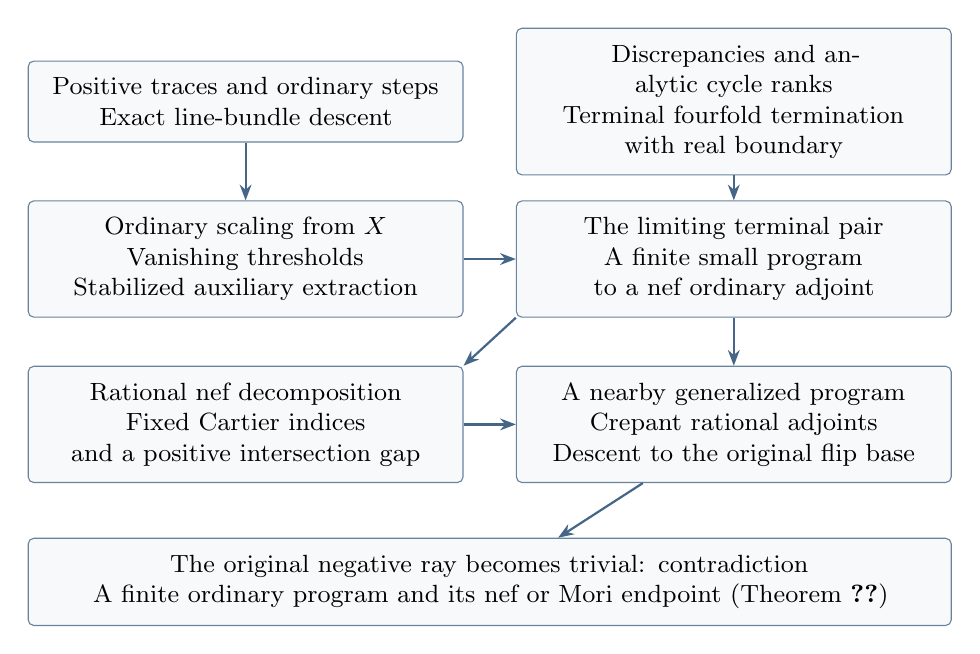
\begin{tikzpicture}[
 box/.style={draw=linkblue!65,rounded corners=2pt,align=center,
 fill=linkblue!3,text width=5.1cm,inner sep=6pt,font=\small},
 edge/.style={-{Stealth[length=2mm]},draw=linkblue!80,thick}]
\node[box] (steps) at (0,0)
 {Positive traces and ordinary steps\\Exact line-bundle descent};
\node[box] (terminal) at (6.2,0)
 {Discrepancies and analytic cycle ranks\\Terminal fourfold termination\\with real boundary};
\node[box] (scaling) at (0,-2)
 {Ordinary scaling from $X$\\Vanishing thresholds\\Stabilized auxiliary extraction};
\node[box] (limit) at (6.2,-2)
 {The limiting terminal pair\\A finite small program\\to a nef ordinary adjoint};
\node[box] (gap) at (0,-4.1)
 {Rational nef decomposition\\Fixed Cartier indices\\and a positive intersection gap};
\node[box] (perturb) at (6.2,-4.1)
 {A nearby generalized program\\Crepant rational adjoints\\Descent to the original flip base};
\node[box,text width=11.3cm] (finite) at (3.1,-6.1)
 {The original negative ray becomes trivial: contradiction\\
 A finite ordinary program and its nef or Mori endpoint
 (Theorem~\ref{thm:finite})};
\draw[edge] (steps)--(scaling);
\draw[edge] (terminal)--(limit);
\draw[edge] (scaling)--(limit);
\draw[edge] (limit.south west)--(gap.north east);
\draw[edge] (gap)--(perturb);
\draw[edge] (limit)--(perturb);
\draw[edge] (perturb)--(finite);
\end{tikzpicture}
\caption{The finite-program argument. The ordinary sequence starts on
$X$. Extraction and the limiting and nearby programs are auxiliary
comparisons. Exact bundle descent preserves the indices used in the
positive intersection gap; the last descent occurs on a common
resolution, as in Figure~\ref{fig:perturbation-descent}.}
\label{fig:dependencies}
\end{figure}


\section{Classes, currents, and exceptional divisors}\label{sec:analytic}

The scaling argument transports one K\"ahler form from the original
space through several birational models.  Its trace need not be smooth,
or even have local potentials without further argument.  We establish
the precise trace relation, its positivity, and the comparison rules
used below.  Equalities between Bott--Chern classes will be distinguished
from equalities between divisors or currents.

\subsection{Pullback of classes}

We use the following cohomological descent theorem.  A space is in
\emph{Fujiki's class $\mathcal C$} if it is bimeromorphic to a compact
K\"ahler manifold.

\begin{lemma}[Pullback and descent]\label{lem:pullback-image}
Let $f:T\to Z$ be a proper surjective morphism with connected fibres between normal
compact analytic spaces with rational singularities.  Suppose that $T$
is in class $\mathcal C$ and that either the general fibre is rationally
connected or $R^jf_*\cO_T=0$ for every $j>0$.  Then
\[
 f^*: \BC(Z)\longrightarrow\BC(T)
\]
is injective, and its image consists exactly of the classes having
degree zero on every $f$-vertical curve.  If $T$ and $Z$ are K\"ahler,
a class on $Z$ is nef if and only if its pullback is nef.
\end{lemma}

\begin{proof}
The pullback assertion is \cite[Lemma~2.39]{HX2026}; nef descent is
\cite[Lemma~2.38]{DHP2024}.  In particular, the first assertion applies
to any proper bimeromorphic morphism between compact spaces with
rational singularities whose source is in class $\mathcal C$: its
general fibre is a point.  For a projective klt log Fano contraction,
relative vanishing supplies the higher-direct-image hypothesis once
rationality of the base has been established.
\end{proof}

\subsection{Positive currents on a normal model}

An $f$-exceptional real divisor is a finite real linear combination of
prime divisors whose images have codimension at least two.
We next give the descent statement needed when an exceptional
correction has either sign.  Pseudo-effectivity requires a positive
current with local plurisubharmonic potentials; we do not assume
that an arbitrary positive current on a singular space has them.

\begin{lemma}[Exceptional descent]\label{lem:positive-descent}
Let $p:U\to T$ be a resolution of a normal compact K\"ahler space,
with $U$ compact K\"ahler.  Let $\alpha\in\BC(T)$ and let $E$ be a
$p$-exceptional real divisor.  If $p^*\alpha+[E]$ is pseudo-effective,
then $\alpha$ is pseudo-effective.  No sign condition on $E$ is needed.
Pseudo-effective classes pull back to resolutions, and nef classes
on $T$ are pseudo-effective.
\end{lemma}

\begin{proof}
Choose a smooth representative $\theta$ of $\alpha$ with local smooth
potentials.  On the smooth compact K\"ahler space $U$, a positive
representative of the given class has the form
\begin{equation}\label{eq:positive-upstairs}
 S=p^*\theta+[E]+\ddc v
\end{equation}
for a global distribution $v$.  Remove from $T$ its singular locus
and the image of the exceptional locus, obtaining a smooth open set
$T^\circ$ whose complement has codimension at least two.  The map
$p$ is an isomorphism there.  Equation~\eqref{eq:positive-upstairs}
gives a global $\theta$-plurisubharmonic function $v^\circ$ on
$T^\circ$.  We do not assert that $v$ is quasi-plurisubharmonic along
$E$.

On a coordinate neighbourhood where $\theta=\ddc\rho$, extend
$\rho+v^\circ$ first across the removed codimension-two subset of
the regular locus, and then across the singular locus.  The first
extension is the plurisubharmonic Hartogs theorem; the second is its
normal-space version of Grauert--Remmert, recalled in
\cite[Section~2.1, pp.~927--928]{CMM2017}. In the latter statement,
every plurisubharmonic function on the regular locus of a normal space
extends uniquely to the whole space; local upper boundedness at the
singular points is not a further hypothesis to be deduced from $v$.
We apply it only after obtaining a plurisubharmonic function on the
entire regular locus. These extensions are unique.
On overlaps their differences are the original smooth
pluriharmonic differences of the functions $\rho$.  Subtracting
$\rho$ therefore gives a global potential $v_T$, and
\[
 \theta+\ddc v_T\geq0
\]
is a current with local plurisubharmonic potentials representing
exactly $\alpha$.  This proves descent, including for signed $E$.

For pullback, compose local plurisubharmonic potentials with the
resolution.  They cannot become identically $-\infty$ on a nonempty
open subset, since a resolution is an isomorphism on a dense open
set.  Thus they define the pulled-back positive current; see
\cite[Section~2.1, p.~928]{CMM2017}.

Finally, if $\alpha$ is nef, then $p^*\alpha$ is nef on $U$.
For a K\"ahler form $\omega_U$, choose positive representatives of
$p^*\alpha+\varepsilon[\omega_U]$.  Their masses are bounded as
$\varepsilon\downarrow0$, so a weak limit is a positive current in
$p^*\alpha$.  On the smooth K\"ahler manifold $U$ it has local
plurisubharmonic potentials.  The first part, with $E=0$, descends
this current to the required class on $T$.
\end{proof}

\subsection{Generalized pairs and negativity}

We recall the generalized-pair language in the form needed here
\cite[Section~2.1 and Definition~2.7]{DHY2023}.  A closed \emph{b-$(1,1)$
current} is a compatible collection of closed $(1,1)$-currents on
proper birational models: pushforward along a morphism between models
recovers the current on the lower model.  It \emph{descends} to a
model $U$ if its trace there and all higher traces have local
potentials, and the classes of the higher traces are pullbacks of
its class on $U$.
It is \emph{b-nef} if that class is nef on some such model.
We also use the relative version for real combinations of line-bundle
data on a carrier projective over a specified base.  Here nefness
means nonnegative degree on curves contracted to that base.  The
structure equation and discrepancy definition below are unchanged.

A generalized pair on $T$ consists of a boundary $B\geq0$, a b-nef
datum $\mathbf M$, and a log resolution $\nu:U\to T$ on which the
datum descends, together with an actual real divisor $B_U$ such that
$\nu_*B_U=B$ and
\begin{equation}\label{eq:generalized-structure}
 [K_U+B_U]+[\mathbf M_U]=\nu^*L,
 \qquad L\in\BC(T).
\end{equation}
The support of $B_U$ may be taken to have simple normal crossings.
Negativity makes this structure boundary unique; passing to higher
resolutions gives the other structure boundaries.  The generalized
log discrepancy of a prime $P$ on such a resolution is
\[
 a(P,T,B+\mathbf M)=1-\operatorname{coeff}_P B_U.
\]
The pair is generalized klt, or \emph{gklt}, if all these discrepancies
are positive, and generalized log canonical, or \emph{glc}, if they
are all nonnegative.  The \emph{gklt locus} is the open subset where
all discrepancies of primes centred there are positive; its
complement is the generalized non-klt locus.  We use the word
\emph{terminal} for an ordinary or
generalized klt pair whose discrepancies at all exceptional primes
are strictly greater than one.  Negative coefficients are permitted
in $B_U$, although the boundary $B$ on the model is effective.
Generalized klt spaces have rational singularities
\cite[Theorem~2.19]{DHY2023}.

The negativity lemma concerns actual divisors, not arbitrary
Bott--Chern classes.  We record also the strict form needed for
fourfold termination.

\begin{lemma}[Negativity and strict comparison]\label{lem:negativity}
\leavevmode
\begin{enumerate}[label=\textup{(\roman*)}]
\item Let $f:T\to Z$ be a proper bimeromorphic morphism of normal
complex spaces and let $E$ be a real Cartier divisor such that $-E$
is $f$-nef.  Then $E\geq0$ if and only if $f_*E\geq0$.
Consequently an $f$-exceptional, $f$-numerically trivial real Cartier
divisor is zero.
\item If, in addition, $f$ has connected projective fibres and
$E\geq0$ is $f$-anti-nef, then every fibre is either contained in
$\Supp E$ or disjoint from $\Supp E$.
\item Consider a nontrivial small birational diagram
\[
 T\xrightarrow{\ f\ }Z\xleftarrow{\ f^+\ }T^+
\]
of normal compact spaces, with projective contractions on both
sides.  Let $B\geq0$ be a real boundary, let $B^+$ be its strict
transform, and suppose the ordinary adjoints
$D=K_T+B$ and $D^+=K_{T^+}+B^+$ are real Cartier, with $-D$ relatively
ample on the left and $D^+$ relatively ample on the right.
The two exceptional loci have the same image $A\subset Z$.  On a
common resolution $p:V\to T$, $q:V\to T^+$,
\begin{equation}\label{eq:ordinary-flip-comparison}
 p^*D-q^*D^+=F,\qquad F\geq0,
\end{equation}
where $F$ is an actual divisor exceptional over both models.
For every prime divisor $P$ over these spaces,
\[
 a(P,T^+,B^+)\geq a(P,T,B),
\]
and the inequality is strict if the centre of $P$ on either side
is contained in that side's exceptional locus.
\item For the diagram in \textup{(iii)}, if $\dim T=4$, then $\dim A\leq1$ and
\[
 \dim\Exc(f)+\dim\Exc(f^+)\geq3.
\]
\item The discrepancy conclusions in \textup{(iii)} also hold for
generalized pairs with the same fixed b-nef datum and transformed
boundaries in a projective small diagram, provided the source log
class has negative degree on every curve contracted on that side,
and the target log class has positive degree on every curve
contracted on the other side.  They hold likewise for a projective divisorial
contraction $f:T\to T'$ when the target boundary is the pushforward,
the b-datum is unchanged, and the source log class has negative
degree on every $f$-vertical curve.  In this divisorial case strictness holds at every prime
whose source centre lies in $\Exc(f)$.
This part also applies when the fixed b-datum is nef only over a
specified base.
\end{enumerate}
\end{lemma}

\begin{proof}
Part~(i) is the analytic negativity lemma
\cite[Lemma~2.5]{HX2026}; apply it to both signs for the last assertion.
For (ii), points of a connected projective fibre can be joined by a
chain of irreducible curves.  If the fibre met both $\Supp E$ and
its complement, some curve in such a chain would meet the support
without being contained in it.  Its intersection with the effective
real Cartier divisor would be strictly positive, contrary to
$f$-anti-nefness.  The assertion for a real Cartier divisor follows
locally from positive combinations of effective rational Cartier
divisors, as explained below.

For (iii), let $G$ be the normalization of the graph in
$T\times_ZT^+$, with projections $p_G,q_G$ and map $h:G\to Z$.
Compatible canonical data give the actual real Cartier divisor
\[
 F_G=p_G^*D-q_G^*D^+.
\]
This difference is defined locally by compatible meromorphic canonical
generators and therefore glues, even when the canonical sheaves were
specified as $\Q$-line bundles.  Smallness makes it exceptional over
both sides.  It is effective by (i), applied over $T$: on a
$p_G$-vertical curve the degree of $-F_G$ is the degree of
$q_G^*D^+$, which is nonnegative.

For every $h$-vertical curve $C$ one has
\begin{equation}\label{eq:graph-strict-degree}
 F_G\cdot C<0.
\end{equation}
Indeed, normalization is finite onto the graph, so the two projections
cannot both contract $C$.  The nonzero degrees contributed by $p_G^*D$
and $-q_G^*D^+$ are both negative.  An effective real Cartier divisor
has nonnegative degree on a curve outside its support.  For completeness,
this fact and its strict pullback analogue hold even if its individual
prime components are not $\Q$-Cartier: locally express it in the real
span of finitely many Cartier divisors.  Vanishing of coefficients
outside its support and nonnegativity of the remaining coefficients
are rational linear conditions.  The resulting rational polyhedral
cone expresses it as a positive real combination of effective
$\Q$-Cartier divisors.  The usual effective Cartier assertions apply
to each term; summing the nonnegative local intersection numbers
gives the asserted global degree inequality.  In particular, the pullback has positive coefficient
at every prime whose centre is contained in the support.

The morphism $p_G$ has connected fibres because $T$ is normal;
hence $h=f p_G$ has connected fibres.  Its fibres are projective
because $G$ is finite over the graph in the fibre product.  Each
point of a positive-dimensional fibre lies on a curve in that fibre.  Equation
\eqref{eq:graph-strict-degree} therefore places the entire fibre in
$\Supp F_G$.  To identify the relevant fibres, suppose $f$ is an
isomorphism over an open subset of $Z$.  There the log divisor on
$T^+$ is pulled back from $Z$, by smallness and agreement in codimension
one.  Relative ampleness excludes an $f^+$-vertical curve there;
projectivity, connectedness and normality then make $f^+$ an
isomorphism there as well.  Interchanging the sides proves that their
exceptional images coincide.  Thus $h^{-1}(A)\subset\Supp F_G$.

Pull $F_G$ back to a resolution on which $P$ appears.  Its coefficient
at $P$ is exactly
$a(P,T^+,B^+)-a(P,T,B)$, with our log-discrepancy convention.
Effectivity gives monotonicity, and the support assertion gives the
claimed strictness.  This proves (iii).

For (iv), a small exceptional locus in a fourfold has dimension at
most two and has positive-dimensional fibres, so its image has
dimension at most one.  Moreover $F_G\ne0$ by
\eqref{eq:graph-strict-degree}.  A component of its support has
dimension three and maps finitely into
$\Exc(f)\times_Z\Exc(f^+)$.  The dimension of this product is at most
the sum of the dimensions of its two factors.  This proves (iv).

For (v), choose a common smooth resolution $p:V\to T$,
$q:V\to T'$ carrying the fixed b-datum and projective over the
common contraction base.  Such a resolution is obtained by taking
projective modifications of the graph that resolve the maps to a
carrier of the datum.  Subtract the actual
structure boundaries to obtain a real Cartier divisor
$F=B_{T,V}-B_{T',V}$.  Its coefficients are the differences of
generalized log discrepancies, and cancellation of the fixed
b-part gives
\[
 [F]=p^*L_T-q^*L_{T'}.
\]
Let $h:V\to Z$ be the morphism to the common contraction base;
in the divisorial case $Z=T'$ and $q=h$.  It is projective by this
choice and has connected fibres because it is bimeromorphic onto
the normal space $Z$.  The boundary-pushforward
condition makes $F$ exceptional over $Z$.  The relative signs of
the log classes give $F\cdot C\leq0$ on every $h$-vertical curve,
with strict inequality whenever $p(C)$ or, in the small case,
$q(C)$ is a curve.  Thus (i) gives $F\geq0$.

If $y$ lies in an exceptional image, a vertical curve downstairs
can be lifted to a curve on $V$ dominating it: use a component of
its projective inverse image and cut by relatively ample
hyperplanes.  Such a curve has negative $F$-degree and hence lies
in $\Supp F$.  Part~(ii) now puts the entire fibre $h^{-1}(y)$ in
the support.  Pullback to a higher resolution has positive
coefficient at every prime centred in this support.  This proves
all the strict discrepancy inequalities, including for a centre
on the flipped side.  No trace current on the normalized graph
is assumed to be Cartier; the actual divisor is constructed from
the structure boundaries on the smooth resolution.
\end{proof}

\subsection{A fixed nef b-part and its traces}

For the finite-program proof, fix a K\"ahler form $h$ on the original
space $X$, and set $H=[h]$.  It defines a positive b-current
$\mathbf H$: for a marked birational model $T$, choose a common
resolution $p:V\to T$, $q:V\to X$ and put
\begin{equation}\label{eq:actual-H-trace}
 \mathbf H_T=p_*q^*h.
\end{equation}
Compatibility on higher resolutions makes this independent of the
choice of resolution \cite[Claim~2.5]{DHY2023}.  Throughout the proof
this is one fixed current datum; we do not replace it by arbitrary
cohomologous currents.  The class of the trace, when it exists, will
be denoted by $H_T$.

\begin{lemma}[The exceptional trace relation]\label{lem:class-trace}
Let $T$ be a normal compact K\"ahler space with rational singularities,
marked birationally to $X$.  Suppose that on a common smooth K\"ahler
resolution $p:V\to T$, $q:V\to X$ there are a class $H_T\in\BC(T)$
and an actual $p$-exceptional real divisor $J_T$ satisfying
\begin{equation}\label{eq:class-trace}
 p^*H_T=q^*H+[J_T].
\end{equation}
Then $J_T\geq0$.  The class $H_T$ and the divisor $J_T$ are unique,
and the correction on a higher resolution is the pullback of $J_T$.

For an effective boundary $B_T$ with real Cartier ordinary adjoint,
the generalized structure boundary for the nef datum $t\mathbf H$ is
\begin{equation}\label{eq:trace-boundary}
 B_{T,V}(t)=p^*(K_T+B_T)-K_V+tJ_T,\qquad t\geq0.
\end{equation}
In particular, decreasing $t$ increases every generalized log
discrepancy.  If the generalized pair is gklt, its ordinary pair is
klt; if all its exceptional log discrepancies exceed one, the
ordinary pair is terminal.

Conversely, suppose $t>0$ and a generalized pair with boundary $B_T$
and this fixed datum $t\mathbf H$ is given by
\eqref{eq:generalized-structure}, with log class $L$ and real Cartier
ordinary adjoint.  Then \eqref{eq:class-trace} holds with
\[
 H_T=\frac{L-[K_T+B_T]}{t}.
\]
\end{lemma}

\begin{proof}
On every $p$-vertical curve, $-J_T$ has the same degree as the nef
class $q^*H$.  Lemma~\ref{lem:negativity}(i) gives $J_T\geq0$.
Subtract two possible relations.  The difference of the correction
divisors is $p$-exceptional and numerically trivial over $T$, hence
zero.  Pullback injectivity from Lemma~\ref{lem:pullback-image} then
gives uniqueness of the class as well.

Pulling back \eqref{eq:class-trace} to a higher resolution gives the
claimed correction there by uniqueness.  Conversely, if the relation
is initially known on a higher resolution $r:V'\to V$, push its
correction down to $V$.  The difference between the upstairs
correction and the pullback of this pushforward is $r$-exceptional
and numerically trivial over $V$, so is zero.  Injectivity of $r^*$
gives the relation on $V$.

Equation~\eqref{eq:trace-boundary} follows by adding $K_V$ and the
fixed nef class $tq^*H$ to its two sides.  Its coefficients give
\[
 a(P,T,B_T+t\mathbf H)
 =a(P,T,B_T)-t\operatorname{coeff}_P J_T
\]
on every sufficiently high resolution.  This proves the discrepancy
assertions.

For the converse, let $B_V$ be the given actual generalized structure
boundary and put $B_V^{\rm ord}=p^*(K_T+B_T)-K_V$.  Both push forward
to $B_T$, so
\[
 J_T=\frac{B_V-B_V^{\rm ord}}{t}
\]
is an actual $p$-exceptional divisor.  Subtract the ordinary log class
from \eqref{eq:generalized-structure} to obtain
\eqref{eq:class-trace}.  This constructs the divisor before applying
negativity; it does not infer a divisor from an arbitrary class
difference.
\end{proof}

The converse is particularly useful for an extraction carrying a
pulled-back generalized log class.  It shows that the divided
difference defining its trace is the same class whenever the marked
model is the same, even if its boundary was obtained at a different
scaling parameter.

\begin{corollary}[Positivity of the trace]\label{cor:big-trace}
Under the hypotheses of Lemma~\ref{lem:class-trace}, the actual trace
$\mathbf H_T$ has local plurisubharmonic potentials and represents
$H_T$.  The class $H_T$ is big.
\end{corollary}

\begin{proof}
The positive current $q^*h+[J_T]$ represents $p^*H_T$.
The proof of Lemma~\ref{lem:positive-descent} constructs a positive
current $S_T$ in $H_T$ with local potentials.  On the big open where
$p$ is an isomorphism and the correction is absent, it agrees with
$p_*q^*h$.  Their difference is a closed current of order zero
supported in codimension at least two.  Such a current vanishes:
after a local embedding it has bidimension
$(\dim T-1,\dim T-1)$, whereas its support has smaller dimension
\cite[Chapter~III, Corollary~2.11]{DemaillyCADG2012}.
Thus $S_T$ is precisely the actual trace in
\eqref{eq:actual-H-trace}.  This step is needed because a trace of
a positive b-current need not have local potentials a priori
\cite[Remark~2.6(ii)]{DHY2023}.

The class $q^*H$ is nef and has positive top self-intersection:
$q^*h$ is semipositive and is positive on the dense open where $q$
is an isomorphism.  By \cite[Theorem~0.5]{DemaillyPaun2004}, it contains
a K\"ahler current $R\geq\delta\omega_V$ for some $\delta>0$ and
some K\"ahler form $\omega_V$.  Fix a K\"ahler form $\omega_T$ and
choose $C>0$ with $p^*\omega_T\leq C\omega_V$.  For
$0<\varepsilon<\delta/C$,
\[
 R+[J_T]-\varepsilon p^*\omega_T\geq0.
\]
Its class is $p^*(H_T-\varepsilon[\omega_T])$.
Lemma~\ref{lem:positive-descent} shows that
$H_T-\varepsilon[\omega_T]$ is pseudo-effective.  Hence $H_T$
contains a K\"ahler current, as required.
\end{proof}

\subsection{Comparison with the same nef datum}

The preceding results supply the positivity needed for scaling.  We
finish with the comparison that later excludes divisorial steps in
the limiting program and identifies the two nef pullbacks in the
final contradiction.

\begin{lemma}[Small-model comparison]\label{lem:small-comparison}
Let $(T,B_T+\mathbf M)$ and $(T',B_{T'}+\mathbf M)$ be generalized
pairs with the same b-nef datum, whose log classes are $L_T$ and
$L_{T'}$.  Suppose the marked birational map $T\dashrightarrow T'$
extracts no divisors and $B_{T'}$ is the pushforward of $B_T$.
On a common sufficiently high resolution $p:V\to T$, $q:V\to T'$, put
\[
 F=B_{T,V}-B_{T',V}.
\]
Then $F$ is an actual divisor exceptional over $T'$, and
\begin{equation}\label{eq:small-comparison}
 p^*L_T-q^*L_{T'}=[F],\qquad
 \operatorname{coeff}_P F
 =a(P,T',B_{T'}+\mathbf M)-a(P,T,B_T+\mathbf M).
\end{equation}
If the map is small, $F$ is exceptional over both models.  In this
case nefness of $L_{T'}$ implies $F\geq0$, and nefness of both log
classes implies $F=0$.  These conclusions also hold relatively over
a common base.  Even without smallness, equality of the pullback classes
in \eqref{eq:small-comparison} implies equality of the structure boundaries.
\end{lemma}

\begin{proof}
Subtract the two structure equations on $V$.  The trace of the fixed
b-datum cancels, giving \eqref{eq:small-comparison}.  At a prime
dominating a divisor on $T'$, the corresponding boundary coefficient
on $T$ is unchanged, so its coefficient in $F$ is zero.  This proves
exceptionality over $T'$.  Smallness gives the same assertion over
$T$.

If $L_{T'}$ is nef, then $-F$ is $p$-nef, because its degree on a
$p$-vertical curve is the degree of $q^*L_{T'}$.  Negativity gives
$F\geq0$.  If $L_T$ is also nef, then $F$ is $q$-nef, so applying
negativity with the opposite sign gives $F\leq0$.  The same proof
uses only relative nefness when the models lie over a common base.
For equal pullback classes, the already constructed exceptional
divisor is relatively numerically trivial, and is zero by
Lemma~\ref{lem:negativity}(i).
\end{proof}

All equalities of pulled-back log classes in this lemma are
cohomological.  Equality of actual currents was used only in the
separate trace-identification argument.  These distinctions allow
the ordinary steps and the generalized auxiliary constructions to
share one fixed nef datum.

\section{Ordinary steps on the given space}\label{sec:absolute}

We construct the contraction and flip of every negative analytic ray in
arbitrary dimension.  The input is an ordinary rational klt pair in the
\emph{global Weil-divisor} category.  Generalized pairs enter only through
the cone and base-point-free theorems; the steps themselves are ordinary.
The main point is to preserve actual line bundles, including their fixed
Cartier indices, rather than only numerical classes.

\subsection{Integral descent}

Bundles are written additively in numerical expressions.  For example,
$L-(K_T+C)$ denotes the rational line bundle obtained from $L$ and the
rational adjoint.  All degrees in the following lemma are degrees on
compact curves contracted by the indicated morphism.

\begin{lemma}[Integral descent]\label{lem:descent}
Let $f:T\to Z$ be a projective bimeromorphic contraction of normal complex
spaces, and let $L$ be a line bundle numerically trivial over $Z$.
Suppose that every point of $Z$ has a neighbourhood $U$ on which there is
an ordinary rational klt pair $(f^{-1}U,C_U)$ with rational adjoint and
\[
 L-(K_{f^{-1}U}+C_U)\quad\text{$f$-nef over $U$}.
\]
Then $f_*L$ is a line bundle and the evaluation map is an isomorphism
\begin{equation}\label{eq:integral-descent}
 f^*f_*L\simeq L.
\end{equation}
In particular the conclusion applies if the local ordinary adjoints are
relatively antiample.  It also applies to a global ordinary rational klt
pair $(T,C)$ whenever $L-(K_T+C)$ is $f$-nef.  Clearing one denominator
therefore descends a rational line bundle as an actual rational line
bundle.
\end{lemma}

\begin{proof}
Fix $z\in Z$ and shrink to a connected Stein neighbourhood $U$ on which
the stated pair is defined.  A line bundle $M$ on $f^{-1}U$ has a
Cartier-divisor representative there: the coherent direct image $f_*M$
has rank one over the nonempty open where $f$ is an isomorphism, so
Cartan's Theorem~A supplies a nonzero section.  Its pullback is a section
of $M$ that is not identically zero, and its zero divisor is Cartier.
This argument takes place over $U$, not on the whole compact space.

Every rational line bundle $N$ on $f^{-1}U$ is also relatively big.
Indeed, choose $q>0$ with $qN$ a line bundle and an $f$-ample line bundle
$A$.  The same direct-image argument gives a nonzero section of
$qN-A$, hence
\[
 N\simq q^{-1}A+q^{-1}E\qquad(E\geq0).
\]
This is relative bigness in the analytic sense
\cite[Definition~2.46]{Fujino2022}.  Apply it to
$N=L-(K_T+C_U)$.  The klt base-point-free theorem gives, after shrinking
around $z$, relative generation of $L^k$ for \emph{every} sufficiently
large integer $k$ \cite[Theorem~6.2 and Remark~6.3]{Fujino2022}.

Choose finitely many such generating sections near the compact fibre
$F=f^{-1}(z)$.  The morphism they define on the projective reduced fibre
$F_{\mathrm{red}}$ is constant on each irreducible component: a
positive-dimensional image would yield a curve with positive degree
against the pullback of the hyperplane bundle, contrary to the
numerical triviality of $L^k$.  Such a curve is obtained by successive
general hyperplane sections of a component.  Connectedness of $F$ makes
the images of all its components the same point.  A linear combination
of the generating sections is consequently nonzero at every point of
$F_{\mathrm{red}}$.

This section is a generator of $L^k$ in the local ring at every point of
$F$: its residue is nonzero, and hence its representing function is a
unit.  This also treats a nonreduced fibre.  Properness allows us to
shrink $U$ away from the image of the section's zero set.  Thus $L^k$ is
trivial on $f^{-1}U$.  Apply the argument to consecutive integers $k$ and
$k+1$, and use one common neighbourhood.  Their quotient trivializes
$L$ itself.  Since $f_*\cO_T=\cO_Z$, on this neighbourhood $f_*L\simeq
\cO_U$, and evaluation is an isomorphism.  These local conclusions give
\eqref{eq:integral-descent} globally.  No additional tensor power enters
the integral conclusion.
\end{proof}

The nef variant is important even when the adjoint has degree zero over
$f$.  For example, if $P=K_T+C$ is a rational klt adjoint, $\ell P$ is
Cartier, and $P$ is numerically trivial over $f$, apply
Lemma~\ref{lem:descent} to $L=\ell P$.  Its difference from the adjoint
is $(\ell-1)P$, so the \emph{same} index $\ell$ descends.

\subsection{Supporting classes and projectivity}

A class is \emph{modified big} if it is the birational pushforward of a big class
\cite[Definition~2.8]{HX2026}. In particular, a big class is modified big.

We use the following consequences of the cone and transcendental
base-point-free theorems \cite[Theorems~1.3 and~1.4]{HX2026}.  For a
compact K\"ahler gklt pair with a descending nef part $\beta$, the cone
$\NA(T)$ is the sum of its adjoint-nonnegative part and rays of rational
curves.  Only finitely many rays are needed when the boundary plus
$\beta$ is big.  If its adjoint class $\alpha$ is nef and the boundary
plus $\beta$ is modified big, there is a Moishezon contraction
$f:T\to Z$ to a normal compact K\"ahler space with $\alpha=f^*\gamma$
for a K\"ahler class $\gamma$ on $Z$.  Neither assertion requires strong
factoriality.  Projectivity in our weaker category will be proved from
the ordinary rational adjoint.

\begin{lemma}[Supports with a K\"ahler margin]\label{lem:absolute-support}
Let $(T,B)$ be an ordinary rational klt pair on a normal compact K\"ahler
space.  Assume that $B$ is $\Q$-Cartier and that $D=K_T+B$ is a rational
line bundle.  If $D$ is not nef, $\NA(T)$ has a $D$-negative extremal ray.
Every such ray $R$ is generated by a rational curve and has a nonempty
relatively open set $\mathcal U_R\subset R^\perp$ of classes satisfying
\begin{equation}\label{eq:absolute-support}
 \alpha\text{ is nef},\qquad
 \NA(T)\cap\alpha^\perp=R,\qquad
 \alpha-c_1(D)\text{ is K\"ahler}.
\end{equation}
\end{lemma}

\begin{proof}
Fix a K\"ahler class $\omega$ and write $d=c_1(D)$.  Cone duality applies
because klt singularities are rational.  The slice
\[
 S=\{v\in\NA(T):\omega\cdot v=1\}
\]
is compact.  Indeed, fix smooth representatives of a basis of $\BC(T)$.
Each is bounded above and below by a multiple of a K\"ahler form, so all
its pairings on $S$ are bounded; the slice is closed.  If $D$ is not nef,
the minimum of $d$ on $S$ is negative.  An extreme point of its minimum
face gives a negative extremal ray.

Fix any such ray and let $r\in S$ be its normalized point.  Choose
$\varepsilon>0$ with $(d+\varepsilon\omega)\cdot r<0$.  The descending
nef part $\varepsilon\omega$ changes no discrepancy, and
$B+\varepsilon\omega$ is big since $B$ is effective and $\Q$-Cartier.
The finite form of the cone theorem gives
\begin{equation}\label{eq:absolute-finite-cone}
 \NA(T)=\NA(T)_{d+\varepsilon\omega\geq0}
       +\sum_{j=1}^{N}\R_{\geq0}[C_j],
\end{equation}
where the $C_j$ are rational curves.  Normalize their classes in $S$
and discard repetitions.  By extremality, $r$ is one of these points,
say $r_1$.  Let $K$ be the convex hull of the others and of
$S\cap\{d+\varepsilon\omega\geq0\}$.  This is compact and excludes
$r$; otherwise extremality of $r$ would fail.

If $K$ is nonempty, strict separation gives a linear functional $h$
with $h(r)=0$ and $h>0$ on $K$, after subtracting a multiple of $\omega$.
Regard it as a Bott--Chern class by duality.  For all sufficiently small
$\delta>0$, $h-\delta d$ is strictly positive on $K$ and at $r$.
Since $S=\operatorname{conv}(\{r\}\cup K)$, it is strictly positive on
$S$, hence K\"ahler.  Thus $\alpha=h/\delta$ has the required properties.
Its positive minimum on $K$ persists under small perturbations in
$R^\perp$; openness of the K\"ahler cone also preserves
$\alpha-d$.  These perturbations give $\mathcal U_R$.  If $K$ is empty,
then $S=\{r\}$ and $-d$ is K\"ahler; a small neighbourhood of $0$ in
$R^\perp$ has the required properties.  This includes the case
$R^\perp=\{0\}$.
\end{proof}

\begin{lemma}[Relative positivity]\label{lem:relative-positivity}
Let $f:T\to Z$ be a proper morphism of compact complex spaces, with $T$
and $Z$ K\"ahler.  Suppose that $L$ is a rational line bundle and
\[
 c_1(L)=\kappa-f^*\gamma,
\]
where $\kappa$ is K\"ahler on $T$ and $\gamma$ is a smooth real
Bott--Chern class on $Z$.  Then $L$ is $f$-ample and $f$ is projective.
Conversely, a normal space projective over a compact K\"ahler space is
compact K\"ahler if it has a global relatively ample line bundle.
\end{lemma}

\begin{proof}
Clear the denominator of $L$ and choose any smooth Hermitian metric
on that line bundle. The Bott--Chern identity says that the difference
between its curvature and the indicated difference of forms is
$\ddc$ of a global smooth function. Adjusting the metric by the
exponential of that function gives the required curvature, with the
same denominator restored at the end. Smooth functions and metrics
here have their normal-space meaning in local embeddings.
On every fibre its curvature is positive.  Positivity of a line bundle
on a compact complex space implies ampleness, and for a proper analytic
map ampleness on every fibre is equivalent to relative ampleness
\cite[Corollary~1.12 and Definition~3.1--Remark~3.2]{FujinoVanishing2026}.
This criterion does not presuppose projectivity and applies to
nonreduced fibres as well.  Existence of the relatively ample line bundle
makes $f$ projective.

For the converse, local relative embeddings give metrics on a relatively
ample bundle with positive curvature in fibre directions.  Glue their
weights by a partition of unity on the base.  The resulting metric
retains that positivity.  Add a sufficiently large multiple of a base
K\"ahler form to its curvature.  The sum is strictly positive; compactness
allows one multiple to work everywhere.
\end{proof}

\subsection{The ordinary contraction and flip}

We can now perform each step and preserve the category.  The next
proposition records both the numerical ranks of the negative contraction
and the actual canonical algebra of a flip.  This description identifies the transformed adjoint as an actual
rational line bundle.

\begin{proposition}[Ordinary negative steps]\label{prop:ordinary-step}
Let $(T,B)$ be an ordinary rational klt pair on a normal compact K\"ahler
space, globally $\Q$-factorial in the Weil-divisor sense, with canonical
sheaf a rational line bundle.  Put $D=K_T+B$.  Every $D$-negative
extremal ray $R\subset\NA(T)$ has a projective contraction $f:T\to Z$
with connected fibres and normal compact K\"ahler target, such that
\begin{equation}\label{eq:ordinary-negative-bc}
 f^*\BC(Z)=R^\perp,\qquad
 \rho(T/Z)=1,\qquad -D\text{ is }f\text{-ample}.
\end{equation}
Here $\rho$ is the rank of global line-bundle degrees on contracted
curves.  The target has rational singularities and
$R^j f_*\cO_T=0$ for $j>0$.  If $\dim Z<\dim T$, this is a Mori fibre
space.  Otherwise $f$ is bimeromorphic, and precisely one of the
following occurs.
\begin{enumerate}[label=\textup{(\roman*)}]
\item The exceptional locus is one prime divisor $E$.  Put $T'=Z$,
$B'=f_*B$ and $D'=K_{T'}+B'$.  Then
\begin{equation}\label{eq:ordinary-divisorial-difference}
 D=f^*D'+eE\qquad(e>0).
\end{equation}
\item The contraction is small.  For an adjoint Cartier index $r>0$,
the intrinsic algebra
\begin{equation}\label{eq:ordinary-flip-algebra}
 \cR_r=\bigoplus_{m\geq0}f_*\cO_T(mrD)
\end{equation}
is locally finitely generated, and $T'=\Proj_Z\cR_r$ is the ordinary
flip.  It has a small projective morphism $f^+:T'\to Z$ with connected
fibres.  Put $B'=\phi_*B$ and $D'=K_{T'}+B'$, where
$\phi:T\dashrightarrow T'$ is the induced small map.  For a sufficiently
divisible choice of $r$ there is an actual isomorphism
\begin{equation}\label{eq:ordinary-tautological}
 \cO_{\Proj_Z\cR_r}(1)\simeq\cO_{T'}(rD').
\end{equation}
In particular $D'$ is a rational line bundle and is $f^+$-ample.
Passing to a sufficiently divisible Veronese leaves $T'$ unchanged.
\end{enumerate}
In both birational cases, $T'$ is compact K\"ahler and globally
Weil-divisor $\Q$-factorial, its canonical sheaf is a rational line
bundle, and $(T',B')$ is klt.  Strong global $\Q$-factoriality is
preserved when imposed on $T$.  A supplied global canonical Weil divisor
is transported to a canonical Weil divisor on $T'$.  No prime divisor is
extracted.  All log discrepancies weakly increase; the increase is strict
for every original prime contracted by the step, and, for a flip, for
every place centred in either exceptional locus.
\end{proposition}

\begin{proof}
Choose $\alpha\in\mathcal U_R$ from Lemma~\ref{lem:absolute-support}
and put $\kappa=\alpha-c_1(D)$.  Insert the descending nef part
$\kappa$ into the ordinary pair.  It changes no discrepancy, while
$B+\kappa$ is big.  Transcendental base-point-freeness gives
$f:T\to Z$ and $\gamma$ K\"ahler with $\alpha=f^*\gamma$.
Thus $c_1(-D)=\kappa-f^*\gamma$, and
Lemma~\ref{lem:relative-positivity} proves projectivity and relative
ampleness.  This establishes projectivity without strong factoriality.
For every curve $C\subset T$,
\begin{equation}\label{eq:ordinary-contracted-curves}
 f(C)\text{ is a point}\quad\Longleftrightarrow\quad
 \alpha\cdot C=0\quad\Longleftrightarrow\quad[C]\in R.
\end{equation}
The rational curve generating $R$ is contracted, so $f$ is nontrivial.

Relative vanishing gives $R^j f_*\cO_T=0$ for $j>0$
\cite[Theorem~5.2]{Fujino2022}; the log Fano base has rational
singularities \cite[Lemma~8.8]{DHP2024}.  Lemma~\ref{lem:pullback-image}
now identifies $f^*\BC(Z)$ with the classes of degree zero on all
vertical curves, which is exactly $R^\perp$.  The global line-bundle
rank is also one, since all those curves are proportional and the
rational line bundle $D$ detects their ray.  This proves
\eqref{eq:ordinary-negative-bc}.  The lower-dimensional case has all
the stated Mori fibre-space properties.  In equal dimension,
connectedness gives generic degree one, so $f$ is bimeromorphic.

\smallskip\noindent
\emph{Divisorial contractions.}
Suppose $E$ is an exceptional prime.  It is $\Q$-Cartier.  If
$E\cdot R\geq0$, it would be $f$-nef, contradicting negativity for a
nonzero effective exceptional divisor.  Thus $E\cdot R<0$.  Every
vertical curve lies in $E$, since an effective $\Q$-Cartier divisor
has nonnegative degree on a curve outside its support.  Every
positive-dimensional projective fibre is covered by curves.  A
zero-dimensional local component of a connected fibre would be isolated,
and the birational form of Zariski's main theorem would make $f$ an
isomorphism there.  Consequently $\Exc(f)=E$.

For a prime Weil divisor $A_Z$ on $Z$, let $A_T$ be its strict transform.
Choose $t\in\Q$ so $(A_T+tE)\cdot R=0$.  The coefficient is rational
by taking the ratio of the two rational degrees on one integral curve.
A Cartier multiple of $A_T+tE$ descends by Lemma~\ref{lem:descent}:
its difference from $D$ is relatively ample.  The descended line bundle
agrees with the corresponding reflexive power of $\cO_Z(A_Z)$ off
$f(E)$, a subset of codimension at least two.  Reflexivity identifies
them everywhere.  Hence every global prime on $Z$ is $\Q$-Cartier.

If a global canonical Weil divisor is given, push it forward.  It agrees
with the canonical sheaf on the big open where $f$ is an isomorphism, so
reflexivity shows that it remains a canonical Weil representative.
Alternatively, start with an invertible reflexive power of $\omega_T$,
adjust it by a rational multiple of $E$ to degree zero, and descend after
clearing denominators.  On the same big open the result is a reflexive
power of $\omega_Z$; hence that power is invertible everywhere.  This
proves the canonical assertion without assuming a global meromorphic
canonical section.

Now $D'$ is a rational line bundle and its canonical identification away
from $E$ gives \eqref{eq:ordinary-divisorial-difference}.  Intersection
with $R$ gives $e>0$.  If $b_E$ is the coefficient of $E$ in $B$, then
\[
 a(E;Z,B')=1-b_E+e>1-b_E=a(E;T,B)>0.
\]
Pullback of the effective divisor $eE$ gives weak increase for all other
log discrepancies.  Thus the target pair is klt.

\smallskip\noindent
\emph{The small canonical model.}
Suppose $f$ is small.  Finite generation of the ordinary relative log
canonical ring \cite[Theorem~1.18]{Fujino2022} gives local finite
generation of \eqref{eq:ordinary-flip-algebra}.  When canonical data are
written as sheaves, this application can be made over each Stein open
in $Z$: nonzero sections of rank-one proper direct images provide the
meromorphic representatives there.  Changing representatives induces
compatible graded isomorphisms of the intrinsic algebra.

The ordinary analytic flip theorem \cite[Theorem~1.14]{Fujino2022}
constructs precisely its relative canonical model.  It has no local
factoriality hypothesis.  Its proof glues the unique local log canonical
models, giving a normal small projective $f^+:T'\to Z$ globally.  The
fibres are connected because $Z$ is normal.  A finite cover of the
compact base permits one common sufficiently divisible Veronese
generated in degree one.  Replace $r$ by that multiple.  The resulting
tautological bundle is relatively ample and agrees with
$\cO_T(rD)$ on the common big open.  Its reflexive extension is
$\cO_{T'}(rD')$, proving \eqref{eq:ordinary-tautological} as an actual
bundle isomorphism.  This also proves that $D'$ is a rational line
bundle.  The relative Proj is invariant under this Veronese operation.
By Lemma~\ref{lem:relative-positivity}, $T'$ is compact K\"ahler.

For a global prime $A'$ on $T'$, transform it to $A$ on $T$ and choose
$t\in\Q$ so $(A+tD)\cdot R=0$.  Descend a Cartier multiple by
Lemma~\ref{lem:descent}.  On $T'$ its pullback agrees on the common big
open with the same multiple of $A'+tD'$.  Reflexivity extends the
identification; since $D'$ is already a rational line bundle, $A'$ is
$\Q$-Cartier.  This proves global Weil-divisor factoriality.  A given
canonical Weil divisor is transported on that common open and then
reflexively.  In the sheaf formulation, repeat the descent argument with
an invertible power of $\omega_T$ adjusted by $tD$; undoing the twist
by $tD'$ proves the rational-line-bundle property of $\omega_{T'}$.

On a common smooth resolution $p:V\to T$, $q:V\to T'$,
Lemma~\ref{lem:negativity} gives the actual discrepancy divisor
\begin{equation}\label{eq:ordinary-small-difference}
 p^*D=q^*D'+F,\qquad F\geq0,
\end{equation}
exceptional over both sides, with the asserted strictness over the
flipping and flipped loci.  This also proves klt preservation.

\smallskip\noindent
\emph{Optional strong factoriality.}
In the divisorial case, take any coherent rank-one reflexive sheaf
$\cF$ on $Z$.  Its reflexive pullback to $T$ is coherent of rank one.
Strong factoriality supplies an invertible reflexive power.  Adjust it
by a rational multiple of $E$, descend as above, and compare off $f(E)$.
A reflexive power of $\cF$ is therefore a line bundle.

In the small case start with such a sheaf $\cF'$ on $T'$.  On a common
smooth resolution put
\[
 \cM=(q^*\cF'/\text{torsion})^{**},\qquad
 \cF=(p_*\cM)^{**}.
\]
Here $\cM$ is a line bundle and $\cF$ is coherent reflexive of rank one;
both give the required transform on the common big open.  An invertible
power of $\cF$, adjusted by a rational multiple of $D$, descends.
Pull back the descended bundle and undo the twist by $D'$.  After
clearing denominators, reflexivity identifies the resulting line bundle
with a reflexive power of $\cF'$.  Thus the strong condition is
preserved.  Only sheaves defined on the whole compact spaces have been
used.

\end{proof}

\subsection{Transport of Bott--Chern classes}

For later scaling we need to transport one fixed nef datum.  The following
construction uses the rank of the negative contraction only.  It makes
no assertion that all Bott--Chern classes on a flipped space come from
the preceding space.

\begin{lemma}[Class transport]\label{lem:class-transport}
For a birational step of Proposition~\ref{prop:ordinary-step}, let
$f':T'\to Z$ mean $f^+$ in the small case and $\id_Z$ in the divisorial
case.  Every $\theta\in\BC(T)$ has a unique expression
$\theta=f^*\eta+s\,c_1(D)$, with $\eta\in\BC(Z)$ and $s\in\R$.
Define
\begin{equation}\label{eq:class-transport}
 \theta'= (f')^*\eta+s\,c_1(D').
\end{equation}
On a common resolution, $p^*\theta-q^*\theta'$ is the class of an
actual divisor exceptional over $T'$.  This rule sends the class of a
global Weil divisor to that of its transform or pushforward.  Moreover,
it propagates the fixed-nef-part trace relation of
Lemma~\ref{lem:class-trace}, with an actual effective exceptional
correction on the new model.  The same conclusions hold for ordinary
real-boundary flips on strongly globally $\Q$-factorial compact K\"ahler
spaces constructed by \cite[Proposition~4.2]{HX2026}.
\end{lemma}

\begin{proof}
Since $D\cdot R\ne0$, subtracting a unique multiple of $c_1(D)$ makes
$\theta$ vanish on $R$.  Equation~\eqref{eq:ordinary-negative-bc} and
pullback injectivity give the unique $\eta$.  On a common resolution
over $Z$ the two pullbacks of $\eta$ agree.  Therefore
\[
 p^*\theta-q^*\theta'
       =s\,[p^*D-q^*D'].
\]
The expression in brackets is the actual exceptional discrepancy
divisor already constructed in the proof of the proposition.

If $\theta=c_1(A)$ for a global Weil divisor $A$, the difference
$p^*A-q^*A'$ is likewise exceptional over $T'$, where $A'$ is its
transform or pushforward.  Subtracting the two identities represents
$q^*(\theta'-c_1(A'))$ by a $q$-exceptional divisor.  That divisor is
numerically trivial over $q$, so negativity in both signs makes it
zero.  Pullback injectivity gives $\theta'=c_1(A')$.

Finally suppose the old trace $H_T$ of a fixed nef class on an earlier
model has, on a common high resolution, the relation
\[
 p^*H_T=p_0^*H+[J_T].
\]
If $H_T=f^*\eta+s\,c_1(D)$, the new correction is the actual divisor
\[
 J_{T'}=J_T-s(p^*D-q^*D'),\qquad
 q^*H_{T'}=p_0^*H+[J_{T'}].
\]
Every old exceptional divisor remains exceptional
over $T'$: neither kind of step extracts divisors.  The resulting
correction $J_{T'}$ is therefore an actual $q$-exceptional divisor.
Its negative is $q$-nef because $p_0^*H$ is nef.  Negativity gives
$J_{T'}\geq0$, and uniqueness and compatibility are those of
Lemma~\ref{lem:class-trace}.

For the stated real-boundary extension, the cited contraction theorem
supplies the negative-side Bott--Chern rank and the ordinary real flip.
The difference $p^*D-q^*D'$ is still an actual exceptional real
discrepancy divisor, by Lemma~\ref{lem:negativity}.  The decomposition,
transport formula, and correction argument above therefore apply
unchanged.  Rationality of $D$ was not used in these arguments.
\end{proof}

\begin{remark}\label{rem:ordinary-continuation}
Proposition~\ref{prop:ordinary-step} starts on the given pair and can be
reapplied after every finite prefix of ordinary steps.  It allows every
negative ray.  Its construction is independent of any termination
claim, and makes no assertion about the positive-side quotient
$\BC(T')/(f^+)^*\BC(Z)$ or about equality of the full Bott--Chern ranks
across a flip.
\end{remark}

\section{Termination for ordinary terminal fourfold pairs}\label{sec:counts}

We prove termination of ordinary flips for compact K\"ahler fourfold
pairs with effective real boundary and log discrepancy $a(E)>1$
for every exceptional place.  Two finite counts
replace projectivity of the ambient fourfold: analytic cycle classes
control contractions, and low-discrepancy places control flipped surfaces.
The bases of successive projective contractions may vary.
We first establish these counts, including their generalized-pair form
needed for extraction later in the proof.

\subsection{Loss of analytic cycle classes}

For a compact complex analytic space $V$ and an integer $k\geq 0$, put
\[
 \begin{split}
 \mathcal C_k(V)
 &:=\operatorname{span}_{\R}\{[S]\in H_{2k}(V,\R):
                  S\subset V\text{ irreducible compact analytic},\ \dim S=k\},\\
 c_k(V)&:=\dim_{\R}\mathcal C_k(V).
 \end{split}
\]
Fundamental classes here use the complex orientation on the regular loci.
Compact analytic spaces admit finite triangulations compatible with any
specified finite collection of closed analytic subsets, with simplicial
dimension at most twice the complex dimension.  Thus $c_k(V)$ is finite.
We justify this topological input after Lemma~\ref{lem:cycle-loss}.
For such a triangulation, Borel--Moore localization is the relative
simplicial-chain sequence for a closed analytic subset and its complement.

If $V$ is K\"ahler and $S$ is such a subspace, then
\begin{equation}\label{eq:positive-cycle}
 \langle[\omega]^k,[S]\rangle=\int_{S_{\mathrm{reg}}}\omega^k>0
\end{equation}
for a K\"ahler form $\omega$ on $V$.  Thus $[S]\neq 0$, including when
$V$ or $S$ is singular.

\begin{lemma}[Cycle loss]\label{lem:cycle-loss}
Let $X\dashrightarrow Y$ be a bimeromorphic transformation of compact
K\"ahler spaces, represented by a proper bimeromorphic diagram.
Suppose it identifies
\[
 U=X\setminus A\simeq Y\setminus B,
\]
where $A$ and $B$ are closed analytic subspaces and $\dim B<k$.
Then there is a surjection
\[
 \mathcal C_k(X)\longrightarrow\mathcal C_k(Y).
\]
If $A$ contains an irreducible compact analytic $k$-dimensional subspace,
then $c_k(X)>c_k(Y)$.

Consequently, in a sequence of bimeromorphic transformations of
$n$-dimensional compact K\"ahler spaces which extract no prime divisors,
only finitely many transformations contract a prime divisor.  A small
transformation preserves $c_{n-1}$.
\end{lemma}

\begin{proof}
The Borel--Moore localization sequence for $B\subset Y$ contains
\[
 H_{2k}(B,\R)\longrightarrow H_{2k}(Y,\R)
 \xrightarrow{\ j_Y^*\ }H_{2k}^{\mathrm{BM}}(U,\R)
 \longrightarrow H_{2k-1}(B,\R).
\]
The outside groups vanish: the real dimension of $B$ is at most $2k-2$.
Thus $j_Y^*$ is an isomorphism.  Compose restriction from $X$ with its
inverse to obtain a linear map
\[
 H_{2k}(X,\R)\xrightarrow{\ j_X^*\ }H_{2k}^{\mathrm{BM}}(U,\R)
 \xrightarrow{\ (j_Y^*)^{-1}\ }H_{2k}(Y,\R).
\]
For an irreducible $k$-cycle $S\subset X$ not contained in $A$, its
restriction is the fundamental class of $S\cap U$.  Closing its image in
$Y$ gives its strict transform: analyticity follows by taking the proper
image of the corresponding strict transform in the given diagram.
The displayed map therefore sends $[S]$ to this transformed cycle class.
It sends $[S]$ to zero when $S\subset A$.

Conversely, no $k$-dimensional subspace of $Y$ is contained in $B$.
Its strict transform in $X$ consequently maps to its fundamental class.
This proves the asserted surjection of cycle spans.  If $S\subset A$
has dimension $k$, its nonzero class, by \eqref{eq:positive-cycle}, is
in the kernel.  This proves the strict inequality.

For a transformation extracting no prime divisor, choose the common
isomorphic open so that the complement in the target has codimension
at least two.  Every contracted source prime lies in the source
complement.  Apply the result with $k=n-1$ at every step.  The
nonnegative integer $c_{n-1}$ cannot decrease infinitely often.  For a
small transformation both complements have codimension at least two,
so applying the result in both directions gives equality.
\end{proof}

This argument does not assert surjectivity on full homology, and does
not compare the Bott--Chern spaces of the two models.

\begin{proof}[Topological justification]
We give the abstract-space reduction for the finite compatible
triangulation used above.  Teissier's compatible Whitney stratification
\cite[Chapter~III, Propositions~1.5 and~2.2.2]{Teissier1982} has finitely
many strata on a compact space.  Choose finitely many analytic charts
$z_j:U_j\hookrightarrow\C^{N_j}$ and nonnegative smooth cutoffs
$\rho_j$ compactly supported in these charts whose positivity sets
cover the space.  Extend $\rho_j$ and $\rho_j z_j$ by zero.  The map
\[
 x\longmapsto\bigl(\rho_j(x),\rho_j(x)z_j(x)\bigr)_j
\]
is a topological embedding into a Euclidean space.  Near a point where
$\rho_j>0$, its components extend smoothly to the ambient chart and the
$j$-th block has the smooth left inverse $(t,w)\mapsto w/t$.
It is therefore locally an ambient smooth embedding, which preserves
the Whitney conditions.  Mather's control data
\cite[Section~7, Proposition~7.1, and Section~8]{Mather1970} and
Goresky's triangulation theorem \cite[Section~5]{Goresky1978} now give
a compatible triangulation, smooth on each stratum.  Compactness makes
it finite, and smoothness on strata gives the dimension bound.
Borel--Moore localization is then the relative simplicial-chain
sequence for a closed analytic subset and its complement.
\end{proof}

\subsection{Low places on compact log smooth data}

We use generalized discrepancies in the sense of
Section~\ref{sec:analytic}.  A place is called exceptional over $X$ when
its center on $X$ has codimension at least two.
The generalized klt statement below supplies the finite extraction set in
Section~\ref{sec:scaling}.  Its coordinate estimate and finite centre-blowup
argument also enter the terminal surface analysis in this section.

\begin{lemma}[Low places and their projective realization]\label{lem:low-places}
Let $(X,B+\bM)$ be a generalized pair on a compact normal complex
space, with effective real boundary of finite support and nef
b-$(1,1)$ data descending to a model projective over $X$.  Fix a projective log resolution $p:W\to X$ carrying those data.
\begin{enumerate}[label=\textup{(\roman*)}]
\item If the pair is generalized klt, there is $\epsilon>0$ such that
every prime divisor over $X$ has log discrepancy at least $\epsilon$,
and only finitely many exceptional places have
\[
 a(E;X,B+\bM)<1+\epsilon.
\]
\item If the pair is generalized terminal and
$b=\max(\{0\}\cup\{\operatorname{coeff}_D B\})$, there are only
finitely many exceptional places with
\[
 a(E;X,B+\bM)<2-b.
\]
\end{enumerate}
In each assertion the finite set of exceptional places can be represented
simultaneously by prime divisors on a smooth model projective over $X$.
In particular, any prescribed finite set of exceptional places with
$a(E;X,B+\bM)\leq 1$ for a generalized klt pair has such a realization.
This conclusion does not use an extraction or termination theorem.
\end{lemma}

\begin{proof}
Let $L\in\BC(X)$ be the generalized log class and let
$M_W=[\bM_W]$ be the nef trace class on $W$.  Write the crepant formula as
\begin{equation}\label{eq:carrier-boundary-count}
 [K_W+\Delta]+M_W=p^*L.
\end{equation}
This is the crepant boundary identity defining generalized
discrepancies; it is an equality of Bott--Chern classes when the nef
data are transcendental.  The boundary $\Delta$ is an actual real
divisor with simple normal crossing support.  Since the nef data
descend to $W$, every further generalized discrepancy is the ordinary
discrepancy for $(W,\Delta)$.  The coefficients of $\Delta$ need not be
nonnegative.  We may enlarge its listed simple normal crossing divisor
by components of coefficient zero.
Here a closed stratum means an irreducible component of an intersection
of listed components; it is smooth, and is the closure of its open
stratum.

We give the local estimate and the realization argument explicitly;
they are the log smooth calculations underlying
\cite[Proposition~2.36]{KM1998} and
\cite[Proposition~2.8]{CT2023}.
Write $\Delta=\sum_j d_jD_j$ and put $w_j=1-d_j$.
Suppose first that every $w_j$ is positive, and set
\[
 \delta=\min\bigl(\{1\}\cup\{w_j\}_j\bigr)>0.
\]
Let $E$ be exceptional over a smooth model with this log smooth
boundary.  At a general point of its center $C$, let $c=\codim C$,
and choose local parameters $x_1,\ldots,x_c$ for $C$ so that the
boundary components containing $C$ are $x_1=0,\ldots,x_r=0$.
For $v=\operatorname{ord}_E$, the Jacobian calculation gives
\begin{equation}\label{eq:coordinate-discrepancy-count}
 a(E;W,\Delta)\geq
 \sum_{j=1}^{r}(1-d_j)v(x_j)+\sum_{j=r+1}^{c}v(x_j).
\end{equation}
Indeed, on a smooth model containing $E$, with local parameter $t$
for $E$, write $x_j=t^{v(x_j)}u_j$ at its general point.  In a top
exterior differential at most one factor can use the term involving
$dt$ that lowers the order by one.  Thus the relative Jacobian has
order at least $\sum_{j=1}^c v(x_j)-1$.  Adding one and subtracting
the boundary orders proves \eqref{eq:coordinate-discrepancy-count}.
The remaining coordinates along $C$ are holomorphic and contribute
no negative orders.

In particular every discrepancy is at least $\delta$: for a divisor
already on the smooth model it is its listed weight, or one if it is
not listed; for an exceptional divisor use
\eqref{eq:coordinate-discrepancy-count}.  If $C$ is not a stratum of
the listed simple normal crossing divisor, then $c>r$.  When $r>0$,
the right hand side is at least $\delta+1$; when $r=0$, it is at
least $c\geq 2\geq\delta+1$.  Hence
\begin{equation}\label{eq:nonstratum-cutoff}
 C\text{ not a stratum}\quad\Longrightarrow\quad
 a(E;W,\Delta)\geq 1+\delta.
\end{equation}

Now fix a place $E$ with discrepancy strictly below $1+\delta$.
If it is not already a divisor on $W$, its center is a stratum by
\eqref{eq:nonstratum-cutoff}.  Blow up that closed stratum.
The center is smooth, the blowup is projective, and the new listed
boundary is again simple normal crossing.  If the center is the
intersection of the components indexed by $J$, then the new exceptional
component has weight
\begin{equation}\label{eq:stratum-weight-sum}
 w_{\mathrm{new}}=\sum_{j\in J}w_j.
\end{equation}
Thus all weights remain at least $\delta$, so the same argument
applies on the next model.  It excludes a non-stratum center at
every stage until $E$ becomes a divisor.

This process is finite.  While $E$ is exceptional, a blowup of its
smooth center of codimension $c\geq2$ changes its ordinary
empty-boundary discrepancy by
\[
 a(E;W_{\mathrm{new}},0)
 =a(E;W_{\mathrm{old}},0)-(c-1)v(\mathcal I_C).
\]
The subtracted quantity is a positive integer, whereas an ordinary
log discrepancy over a smooth space is a positive integer.
Consequently only finitely many such blowups are possible.
Thus $E$ is obtained by successive stratum blowups, which is the
meaning of a \emph{toroidal place} here.  This also realizes it on a projective model without first assuming
that the original model on which $E$ was given was projective over $X$.

For completeness, there are only finitely many such toroidal places.
A toroidal prime over a fixed irreducible stratum is determined by a
primitive nonzero vector $(m_j)_{j\in J}$ of nonnegative integers
in the normal boundary directions.  Its discrepancy is
\begin{equation}\label{eq:monomial-discrepancy-count}
 \sum_{j\in J}m_jw_j.
\end{equation}
These statements follow also directly from the successive stratum
blowups: a blowup inserts the sum of the relevant coordinate rays,
and the discrepancy transforms by \eqref{eq:stratum-weight-sum}.
The vector determines the monomial order and is unchanged when a
boundary equation is multiplied by a unit.  There are finitely many
irreducible strata on the compact model.  Since each $w_j\geq\delta$,
an upper bound $T$ on \eqref{eq:monomial-discrepancy-count} bounds
every $m_j$ by $T/\delta$.  This leaves finitely many vectors and
hence finitely many places.  Add the finitely many prime divisors
already on $W$ which are exceptional over $X$.

For a generalized klt pair, all weights in
\eqref{eq:carrier-boundary-count} are positive.  The preceding
argument with $\epsilon=\delta$ proves \textup{(i)} and its projective
realization assertion.  In particular $a\leq1$ lies strictly below
$1+\delta$.

No rationality of the weights was used: their fixed positive minimum
bounds the nonnegative integer vectors.  Thus the conclusion applies
to real boundaries and real nef data.

For a generalized terminal pair, the coefficient of every
$p$-exceptional component in $\Delta$ is negative, since its
log discrepancy is greater than one.  The other coefficients are
the original boundary coefficients and are at most $b<1$.
All the weights on $W$ are therefore at least $1-b$.
Repeat the argument with $\delta=1-b$ and $T=2-b$ to prove
\textup{(ii)}.  Subsequent stratum blowups preserve this lower bound
by \eqref{eq:stratum-weight-sum}.

Finally, to represent the entire finite set at once, take the
dominating component of the fiber product of the finitely many
projective realizations over $W$, normalize, and resolve projectively.
The strict transforms of the designated prime divisors remain
divisors on this common model.  Its composite map to $X$ is projective.
\end{proof}

\begin{remark}\label{rem:strict-low-cutoff}
The strict inequalities in Lemma~\ref{lem:low-places} are necessary.
For example, in $\mathbf P^n$, $n\geq3$, let $H$ be a hyperplane
with coefficient $b\in[0,1)$.  Blowing up any codimension-two linear
subspace contained in $H$ gives log discrepancy $2-b$ for
$(\mathbf P^n,bH)$.  There are infinitely many such places, although
this pair is terminal.  With empty boundary their discrepancy is two.
Below we count places strictly below a threshold and use a step at
which a place reaches that threshold to obtain a strict decrease.
\end{remark}


\subsection{Surface centres of low-discrepancy places}

The terminal termination argument must allow many places of discrepancy
below two above a moving boundary surface.  After recalling smoothness in
codimension two, Lemma~\ref{lem:terminal-low-centres} identifies the infinite
families that will be harmless.  Excluding only
the first blowup above each surface would be incorrect; the correction
in \cite[Proposition~3.1 and Lemma~3.2]{Fujino2005Addendum} is essential.

\begin{lemma}\label{lem:terminal-codim-two}
Let $(T,\Phi)$ be an ordinary klt pair on a normal complex fourfold,
with effective real boundary, $K_T$ a $\Q$-line bundle, and
$a(E;T,\Phi)>1$ for every exceptional prime divisor $E$ over $T$.
Then $T$ is smooth in codimension two.
\end{lemma}

\begin{proof}
Dropping the effective boundary shows that $T$ has terminal
singularities.  Suppose its singular locus has a codimension-two
component.  Near a general smooth point of this component choose a
holomorphic projection to $\C^2$ submersive along it.  Take a general
fibre transverse both to the regular locus and, on a fixed log
resolution, to the exceptional divisor and its strata.  These
transversality conditions hold after shrinking and choosing a general
value.  The resulting surface is a complete intersection in the
Cohen--Macaulay space $T$, since klt singularities are rational, and is
regular outside isolated points.  It is therefore normal.

Adjunction of a local Cartier pluricanonical power, first on the regular
locus and then by reflexivity, restricts the relative canonical equality
to the surface resolution.  All its exceptional discrepancy coefficients
are positive.  A normal surface germ with this property is smooth.
Indeed, negative definiteness of the exceptional intersection matrix
shows that a positive exceptional discrepancy divisor has negative
intersection with some exceptional curve.  That curve has negative
canonical degree; adjunction makes it a smooth rational $(-1)$-curve.
Contract it smoothly and repeat.  The remaining discrepancy coefficients
stay positive by pushforward.  Eventually no exceptional curve remains,
and the proper bimeromorphic map to the normal surface is an isomorphism.

On the other hand, a slice of a singular fourfold point by two equations
has embedding dimension at least the ambient embedding dimension minus
two, and hence greater than two.  The chosen surface is singular there,
a contradiction.
\end{proof}

\begin{lemma}\label{lem:terminal-low-centres}
Let $(T,\Phi)$ be an ordinary klt pair on a compact normal complex
fourfold, where $\Phi\geq0$ is real and
$a(E;T,\Phi)>1$ for every exceptional prime divisor $E$ over $T$.
Apart from finitely many exceptional places, every exceptional place with
$a(E;T,\Phi)<2$ has centre a surface $S\subset T$ with the following
properties: $T$ and the reduced support of $\Phi$ are generically smooth
along $S$, exactly one positive boundary component contains $S$, and,
if its coefficient is $b$, then
\[
 a(E;T,\Phi)\geq 2-b.
\]
All places above such a surface are allowed in this conclusion, not just
the exceptional divisor of its first blowup.
\end{lemma}

\begin{proof}
Choose a log resolution on which the positive strict boundary components
are smooth and mutually disjoint.  Starting with simple normal crossing
support, blow up intersections of the positive components to separate
them.  Every exceptional crepant coefficient is negative by terminality.
Thus the only positive components on this resolution are those disjoint
strict transforms, with their original coefficients.

Consider a place not already on the resolution.  At its general centre,
apply \eqref{eq:coordinate-discrepancy-count}, dropping negative boundary
coefficients.  A centre of codimension at least three has log discrepancy
at least $3-b>2$, if it lies in a positive component of coefficient $b$,
and at least three otherwise.  A codimension-two centre outside the
positive support has log discrepancy at least two.  Thus a place with
$a<2$ has codimension-two centre in one positive component, and its log
discrepancy is at least $2-b$.

If this centre lies in the exceptional locus, it is an irreducible
component of the intersection of that positive component and an
exceptional divisor.  There are finitely many such centres on the compact
resolution.  We check that each supports only finitely many places with
$a<2$.  It suffices to retain only the smooth component of coefficient
$b$, since deleting the negative coefficients lowers discrepancies.
Make this reduction once on the fixed resolution; on subsequent blowups
retain all exceptional coefficients in the crepant boundary.
Blow up the fixed centre at its general point.  Unless the given place
has appeared, the same estimate forces its next centre to be the
intersection of the positive strict transform and the new exceptional
divisor.  Indeed, the strict transform of the positive divisor maps isomorphically
to that divisor near the generic point of the original centre, because
the centre is Cartier within it. A codimension-two centre over that
generic point must therefore be this unique intersection. A proper
subset has codimension at least three and discrepancy at least $3-b$;
a centre outside the positive divisor has discrepancy at least two.
Thus no other branch is possible. The process reaches the given place
after finitely many blowups, by the decreasing positive integer
empty-boundary discrepancy used in Lemma~\ref{lem:low-places}.
For this reduced pair, the $k$th exceptional divisor on the branch has
crepant coefficient $-k(1-b)$ and log discrepancy
\[
 1+k(1-b),\qquad k=1,2,\ldots.
\]
Indeed, the first coefficient is $b-1$, and blowing up the intersection
of the newest exceptional divisor with the coefficient-$b$ strict
transform changes $-k(1-b)$ to $b-k(1-b)-1=-(k+1)(1-b)$.
Thus only
$k<1/(1-b)$ can occur before the cutoff two is reached.  This proves
finiteness over every fixed exceptional centre.  These generic blowups
are realized globally by blowing up the closures of the centres.

Add the finitely many exceptional primes on the chosen resolution.
All other centres under consideration lie outside its exceptional locus
at their general points, where the resolution is an isomorphism.  Their
images are precisely the surfaces described in the statement.
\end{proof}

We now have the two counts needed for termination.  A flipped surface
will give a place whose discrepancy strictly increases into a fixed
finite set.  Once such surfaces disappear, a compact surface-class rank
will decrease at every remaining step.

\subsection{Real terminal pairs}

\begin{proposition}\label{prop:terminal-real-four}
Let $(T_0,\Phi_0)$ be an ordinary klt pair on a normal globally
$\Q$-factorial compact K\"ahler fourfold, with $K_{T_0}$ a
$\Q$-line bundle and effective real boundary.  Suppose
$a(E;T_0,\Phi_0)>1$ for every exceptional prime divisor $E$ over $T_0$.
Every sequence of ordinary $(K_{T_i}+\Phi_i)$-flips starting at this
pair terminates, provided all models are normal globally $\Q$-factorial
compact K\"ahler fourfolds, each $K_{T_i}$ is a $\Q$-line bundle, and
each flip is given by projective small contractions
\[
 T_i\xrightarrow{\ f_i\ }Z_i
 \xleftarrow{\ f_i^+\ }T_{i+1}
\]
with $-(K_{T_i}+\Phi_i)$ relatively ample for $f_i$ and
$K_{T_{i+1}}+\Phi_{i+1}$ relatively ample for $f_i^+$.
Here $\Phi_{i+1}$ is the strict transform of $\Phi_i$.
No pseudo-effectivity or bigness assumption is required.
\end{proposition}

\begin{proof}
By Lemma~\ref{lem:negativity}, discrepancies do not decrease, and they
increase strictly for a place centred in either exceptional locus.
Since the maps are small, the exceptional places are the same on all
models.  Thus every pair remains terminal in the stated sense, and its
ambient fourfold is smooth in codimension two by
Lemma~\ref{lem:terminal-codim-two}.

Write the distinct positive coefficients of the boundary in decreasing
order.  We successively remove, by discarding finitely many initial
steps, every flipping and flipped surface contained in a component of
each coefficient.  After the positive coefficients we treat the value
zero, at which stage every flipped surface is considered.

\smallskip\noindent
\emph{Eliminating flipped surfaces.}
Fix the current coefficient $b$, and suppose that no flipping or flipped
surface is contained in a component of coefficient greater than $b$.
For $b=0$ assume that all positive coefficients have already been treated.
If $S$ is a flipped surface contained in a coefficient-$b$ component,
or any flipped surface when $b=0$, blow it up at its general point.
The exceptional prime $E$ has new log discrepancy
\begin{equation}\label{eq:surface-witness-values}
 a(E;T_{i+1},\Phi_{i+1})
   =2-\sum_{l=1}^{s}b_l\operatorname{mult}_{S}\Phi_{l,i+1},
 \qquad 1<a(E;T_{i+1},\Phi_{i+1})\leq2-b,
\end{equation}
where $\Phi_{l,i+1}$ are the positive prime boundary components and
$b_l$ their fixed coefficients.  The blowup place is defined globally
by blowing up the closed surface and resolving; its generic point
suffices for this computation.

The values in \eqref{eq:surface-witness-values} belong to a finite set,
even for irrational coefficients.  Indeed, terminality gives
\[
 \sum_l b_l\operatorname{mult}_{S}\Phi_{l,i+1}<1,
 \qquad
 0\leq\operatorname{mult}_{S}\Phi_{l,i+1}<1/b_l.
\]
Each multiplicity is an integer, and there are finitely many positive
components.  We use no discreteness assertion for all discrepancies.

Strictness in Lemma~\ref{lem:negativity} gives
$a(E;T_i,\Phi_i)<2-b$.  Its discrepancy on the first model of the
current tail is therefore also strictly below $2-b$.  By
Lemma~\ref{lem:terminal-low-centres}, outside a finite set such a place
would initially have a surface centre in one boundary component of
coefficient $c$, with discrepancy at least $2-c$.  Necessarily $c>b$.
That centre persists as a surface in this component at every later
step: at each step the map is an isomorphism at its general point,
since otherwise the centre itself would be a flipping surface in a
higher-coefficient component.  It cannot become a flipped surface
either, by the same higher-coefficient exclusion.  Thus it cannot be
the place just constructed.  All these witness places belong to a
fixed finite set.

Each member of that finite set is used only finitely often.  Between
uses its discrepancy does not decrease, and at each use it strictly
increases to one of the finitely many values
\eqref{eq:surface-witness-values}.  Consequently only finitely many
steps have a flipped surface of the current kind.  Pass beyond them.

\smallskip\noindent
\emph{Eliminating flipping surfaces inside the boundary.}
Suppose $b>0$.  Fix a coefficient-$b$ component and normalize its
transforms on the two sides of a flip.  Denote the normalizations by
$D_i^\nu,D_{i+1}^\nu$, and normalize their common image in $Z_i$ to
obtain $B_i$.  The induced maps to $B_i$ are proper and bimeromorphic.
They are isomorphisms away from the inverse image of the common
exceptional image in $Z_i$, whose dimension is at most one by
Lemma~\ref{lem:negativity}.  Finite normalization preserves this bound.
On $D_{i+1}^\nu$ its inverse image also has dimension at most one,
because no flipped surface is contained in the boundary component.

Every compact surface in $B_i$ has a strict transform on $D_i^\nu$,
so pushforward gives a surjection
\[
 \mathcal C_2(D_i^\nu)\longrightarrow\mathcal C_2(B_i).
\]
On the other side, Borel--Moore localization along the exceptional
subset of dimension at most one makes restriction in degree four
injective.  Compatibility with proper pushforward and the common
isomorphic open therefore gives an injection
\[
 \mathcal C_2(D_{i+1}^\nu)\lhook\joinrel\longrightarrow
 \mathcal C_2(B_i).
\]
These are assertions about surface spans; no surjectivity on the full
fourth homology of the negative side is needed. Only compact analytic
topology is used on the normalized components and their common image;
the positivity needed next comes from the ambient Kähler fourfold.

If a flipping surface lies in this boundary component, a surface above
it on $D_i^\nu$ maps to a set of dimension at most one in $B_i$.
Its class is nonzero: its image in $T_i$ is a surface, and the square
of a K\"ahler class on $T_i$ has strictly positive integral over it.
One may compute this integral on a resolution of the surface.
The finite normalization has positive generic degree on this surface,
so the same nonvanishing holds upstairs.  Its class is a nonzero
kernel vector in the displayed surjection.  Hence
\[
 c_2(D_i^\nu)\geq c_2(D_{i+1}^\nu),
\]
with strict inequality whenever the component contains a flipping
surface.  Summing over the finitely many coefficient-$b$ components
shows that only finitely many such steps occur.  This completes the
induction at $b$.

\smallskip\noindent
\emph{The remaining flips.}
After the positive coefficients have been treated, perform the
flipped-surface argument with $b=0$.  No flipped surface remains.
For every remaining flip, Lemma~\ref{lem:negativity} gives
\[
 \dim\Exc(f_i)+\dim\Exc(f_i^+)\geq3.
\]
Smallness bounds both dimensions by two, so $\Exc(f_i)$ contains a
surface and $\dim\Exc(f_i^+)\leq1$.  Apply
Lemma~\ref{lem:cycle-loss} with $k=2$ to the common isomorphic open.
It gives $c_2(T_i)>c_2(T_{i+1})$ at every remaining step, impossible
for an infinite sequence of nonnegative integers.
\end{proof}

The algebraic discrepancy and cycle-count strategy originates in
\cite[Theorem~5-1-15 and Lemmas~5-1-16--5-1-17]{KMM1987}
and \cite{Fujino2004,Fujino2005Addendum}.
The proof above supplies the real-boundary argument and uses compact
analytic cycle classes with K\"ahler positivity.  It applies those
geometric tools one step at a time, without a common projective base.

\begin{corollary}\label{prop:terminal-four}
Let $X_0$ be a normal globally strongly $\Q$-factorial compact
K\"ahler fourfold with terminal singularities.
Every sequence starting at $X_0$ of ordinary empty-boundary negative
divisorial contractions and flips, with the projectivity and compact
K\"ahler conclusions of Proposition~\ref{prop:ordinary-step}, terminates.
No pseudo-effectivity hypothesis is required for this assertion about
birational sequences.
\end{corollary}

\begin{proof}
For flips, terminality persists by Lemma~\ref{lem:negativity}.
For a divisorial contraction, \eqref{eq:ordinary-divisorial-difference}
gives $K_{X_i}=f^*K_{X_{i+1}}+eE$ with $e>0$.
The lost prime has target log discrepancy $1+e>1$; every other
exceptional place has target discrepancy at least its source
discrepancy, which was greater than one.  Thus terminality persists
throughout the sequence.
Lemma~\ref{lem:cycle-loss} with $k=3$ bounds the number of divisorial
steps.  Any infinite sequence would therefore have a tail consisting
only of flips, contrary to Proposition~\ref{prop:terminal-real-four}
with zero boundary.
\end{proof}

\section{Scaling and a limiting terminal pair}\label{sec:scaling}

We now construct a particular ordinary program on the pair of
Theorem~\ref{thm:finite}.  If that program were infinite, we would obtain
strongly \(\Q\)-factorial auxiliary models carrying nef generalized
adjoints and a decreasing sequence of effective boundaries.  Their limit
will be an ordinary terminal pair.  These auxiliary extractions are used
only to compare the original program with a terminating one; the
original program starts on \(X\).

Fix a smooth Kähler form \(h\) on \(X\), with class \(H\), large enough
that \(K_X+\Delta+H\) is nef.  Throughout this section
\(\mathbf H\) denotes the fixed b-nef datum obtained by pulling back
this very form.  On subsequent models its trace class is denoted by
\(H_T\), as in Lemma~\ref{lem:class-trace}.  We do not replace the
fixed datum by arbitrary cohomologous current representatives.

\subsection{Constructing the scaling program}

\begin{proposition}\label{prop:scaling-construction}
Let \((X,\Delta)\) satisfy the hypotheses of Theorem~\ref{thm:finite}.
There is an ordinary negative-ray program, finite or infinite,
\[
 (X,\Delta)=(X_0,\Delta_0)\dashrightarrow
 (X_1,\Delta_1)\dashrightarrow\cdots,
\]
in the same global Weil-divisor \(\Q\)-factorial compact Kähler
category.  It stops when the ordinary adjoint is nef or a negative ray
has a Mori fibre contraction.  Put
\[
 D_i=K_{X_i}+\Delta_i,\qquad
 L_i(t)=D_i+tH_i,\qquad H_i=H_{X_i},\qquad \lambda_{-1}=1.
\]
At every stage before stopping there is a parameter
\(0<\lambda_i\leq\lambda_{i-1}\) and a contracted extremal ray
\(R_i\) such that
\[
 D_i\cdot R_i<0,\qquad L_i(\lambda_i)\cdot R_i=0,
 \qquad L_i(\lambda_i)\text{ is nef}.
\]
The generalized pairs \((X_i,\Delta_i+t\mathbf H)\) are gklt for
\(0\leq t\leq\lambda_{i-1}\).  A birational step is crepant for the
data at \(t=\lambda_i\), and discrepancies do not decrease across
that step for any \(0\leq t\leq\lambda_i\).
\end{proposition}

\begin{proof}
On \(X_0\), the nef datum descends, so its addition changes no
discrepancies.  Thus all the initial generalized pairs are gklt.
Suppose the assertions have been established through \(X_i\).
If \(D_i\) is nef, stop.  Otherwise define
\[
 \lambda_i=\min\{t\in[0,\lambda_{i-1}]:L_i(t)\text{ is nef}\}.
\]
The set is nonempty by induction and is closed and convex.  Its minimum
is positive because \(D_i\) is not nef.

We first find a ray at this threshold.  Choose
\(t_k\uparrow\lambda_i\) with \(\lambda_i/2<t_k<\lambda_i\).
The generalized cone theorem gives an extremal ray negative for
\(L_i(t_k)\).  Since \(L_i(\lambda_i)\) is nef, that ray is also
negative for \(L_i(\lambda_i/2)\).  The trace \(H_i\) is big by
Corollary~\ref{cor:big-trace}.  Hence
\(\Delta_i+(\lambda_i/2)H_i\) is big, and the cone theorem gives
only finitely many negative rays for this latter generalized pair
\cite[Theorem~1.3]{HX2026}.  One ray \(R_i\) therefore occurs for
infinitely many \(k\).  On this fixed ray, continuity gives
\(L_i(\lambda_i)\cdot R_i=0\).  Moreover
\(H_i\cdot R_i>0\), so \(D_i\cdot R_i<0\).

Apply Proposition~\ref{prop:ordinary-step} to this ordinary negative
ray, and denote its contraction by \(f_i:X_i\to Z_i\).  A fibre
contraction gives the stopping alternative.  Otherwise make the
ordinary divisorial step or flip.  Lemma~\ref{lem:class-transport}
transports the trace \(H_i\) to \(H_{i+1}\) while preserving its
relation to the fixed b-datum.  By Lemma~\ref{lem:pullback-image}, the
class \(L_i(\lambda_i)\) descends to \(Z_i\).  Its descended class
is nef, and its pullback on the new model is
\(L_{i+1}(\lambda_i)\).  Thus the two threshold classes have equal
pullbacks on a common resolution.  Their difference is represented by
the actual exceptional discrepancy divisor, which vanishes by
negativity as in Lemma~\ref{lem:small-comparison}.  The step is
consequently generalized crepant at the threshold.

For completeness, this also proves the induction on singularities.
On a common resolution, the log discrepancy at each prime \(E\) is
affine in \(t\).  Its difference across the step is zero at
\(t=\lambda_i\) and is the ordinary discrepancy increase at zero.
Consequently
\begin{align}
 &a(E,X_{i+1},\Delta_{i+1}+t\mathbf H)
       -a(E,X_i,\Delta_i+t\mathbf H)\notag\\
 &\qquad=\left(1-\frac{t}{\lambda_i}\right)
     \bigl(a(E,X_{i+1},\Delta_{i+1})-a(E,X_i,\Delta_i)\bigr)
     \geq0\label{eq:scaling-interpolation}
\end{align}
for \(0\leq t\leq\lambda_i\).  The generalized pairs on this
interval remain gklt, and the new upper-threshold class is nef.  The
ordinary steps preserve all the stated properties of the original
category by Proposition~\ref{prop:ordinary-step}.
\end{proof}

\subsection{An infinite program has vanishing thresholds}

We record first why an infinite program has a tail consisting only of
flips.  Use the cycle-space notation of Lemma~\ref{lem:cycle-loss}:
\(c_3(T)\) is the dimension of the span of compact analytic
three-dimensional cycle classes in \(H_6(T,\R)\).  It is finite.
A small modification of fourfolds is an isomorphism away from sets of
dimension at most two, so that lemma, applied in both directions,
preserves \(c_3\).  A divisorial contraction strictly lowers it: an
exceptional divisor has a nonzero cycle class, detected by integration
of the cube of a Kähler form, and maps to a set of dimension at most
two.  Therefore only finitely many divisorial steps occur.

\begin{lemma}\label{lem:scaling-zero}
If the program of Proposition~\ref{prop:scaling-construction} is
infinite, then \(\lambda_i\to0\).
\end{lemma}

\begin{proof}
Fix \(0<\epsilon<1\) and a resolution \(\nu:U\to X\).  Consider the
compact segment of generalized data
\[
 \mathcal P_\epsilon
 =\{(\Delta,t\nu^*H):\epsilon\leq t\leq1\}
 \subset \operatorname{Div}_{\R}(X)\times\BC(U).
\]
The upstairs nef data here are the pullbacks of the fixed smooth form.
Every pair in this segment is gklt, its upstairs class is nef, and its
boundary-plus-trace is modified big, since \(tH\) is Kähler on \(X\).
This real segment is allowed in the finiteness theorem for weak log
canonical models \cite[Theorem~5.15]{HX2026}; neither rationality of
\(H\) nor strong \(\Q\)-factoriality of \(X\) is required there.

Let \(\phi_i:X\dashrightarrow X_i\) be the accumulated map, and
suppose \(\lambda_i\geq\epsilon\).  It is a weak log canonical
model of the original generalized pair at parameter \(\lambda_i\).
Indeed, it extracts no divisors, its target adjoint is nef, and
discrepancies do not decrease: apply
\eqref{eq:scaling-interpolation} to every preceding step at the fixed
parameter \(\lambda_i\), which is no larger than any preceding
threshold.  On a common resolution the original adjoint is the
pullback of the target nef class plus an effective exceptional
divisor.  Pseudo-effectivity descends by
Lemma~\ref{lem:positive-descent}, so the original data belong to the
pseudo-effective portion of \(\mathcal P_\epsilon\).

The finiteness conclusion concerns the maps \(\phi_i\), up to
isomorphisms of their targets commuting with the maps from \(X\).
These marked maps are pairwise distinct in the flip tail.  In fact,
given two stages, an exceptional prime has strictly increasing
ordinary discrepancy at the first intervening flip by
Lemma~\ref{lem:negativity}, and later steps
cannot decrease it.  A target isomorphism compatible with the marking
would identify the transformed boundary and all its discrepancies,
a contradiction.  This is also the distinction used in the proof of
\cite[Theorem~5.16]{HX2026}.

There are therefore only finitely many \(i\) with
\(\lambda_i\geq\epsilon\).  Since \(\epsilon>0\) was arbitrary,
the thresholds tend to zero.
\end{proof}

An infinite program would thus provide nef generalized adjoints with
arbitrarily small nef parts.  We next put their nonterminal places on
auxiliary models, so that the boundary can be allowed to converge on
one fixed space.

\subsection{Stabilizing the extractions}

\begin{proposition}\label{prop:terminal-limit}
Suppose the program of Proposition~\ref{prop:scaling-construction} is
infinite.  After discarding finitely many stages, there are proper
bimeromorphic morphisms
\[
 \mu_i:Y_i\longrightarrow X_i
\]
with \(Y_i\) strongly \(\Q\)-factorial and compact Kähler, and
effective real boundaries \(\Theta_i\), with the following properties.
\begin{enumerate}[label=\textup{(\roman*)}]
\item The natural maps between the \(Y_i\) are isomorphisms in
codimension one, and
\begin{equation}\label{eq:extracted-nef-adjoint}
 Q_{i,Y_i}:=K_{Y_i}+\Theta_i+\lambda_iH_{Y_i}
       =\mu_i^*L_i(\lambda_i)
\end{equation}
is nef.  Each ordinary pair \((Y_i,\Theta_i)\) is klt and terminal.
\item On a fixed first model \(Y=Y_{i_0}\), write
\(\Theta_{i,Y}\) for the strict transform of \(\Theta_i\).
These boundaries have a fixed finite containing support and decrease
coefficientwise to an effective real boundary \(\Theta_Y\).
The ordinary pair \((Y,\Theta_Y)\) is klt and terminal.
\item The strict transform of \(\Theta_Y\) on each \(Y_i\)
pushes forward to \(\Delta_i\) under \(\mu_i\).
\end{enumerate}
Here terminal means that every exceptional prime has log discrepancy
strictly greater than one.
\end{proposition}

\begin{proof}
Discard the finitely many divisorial steps.  All remaining maps
\(X_i\dashrightarrow X_{i+1}\) are small.  For each such \(i\), put
\[
 \mathcal E_i=\{E\text{ exceptional over }X_i:
      a(E,X_i,\Delta_i+\lambda_i\mathbf H)\leq1\}.
\]
The fixed nef datum has a carrier projective over \(X_i\): take a
common resolution of the finitely many preceding projective ordinary
step diagrams.  For a flip its graph is projective over either side,
so this construction and a further projective log resolution retain
projectivity over \(X_i\).  On this resolution the datum is the
pullback of \(h\).  Lemma~\ref{lem:low-places} therefore makes
\(\mathcal E_i\) finite.  It allows real coefficients and counts
places of log discrepancy exactly one as well as those below one.

Smallness identifies the primes exceptional over successive
\(X_i\).  Their log discrepancies at the current threshold agree by
crepancy.  On the new model, decreasing the coefficient of the nef
part increases discrepancies: in the trace formula of
Lemma~\ref{lem:class-trace}, the correction divisor is effective.
Thus, for every such prime,
\begin{equation}\label{eq:decreasing-extraction-sets}
 \begin{split}
 a(E,X_{i+1},\Delta_{i+1}+\lambda_{i+1}\mathbf H)
 &\geq a(E,X_{i+1},\Delta_{i+1}+\lambda_i\mathbf H)\\
 &=a(E,X_i,\Delta_i+\lambda_i\mathbf H).
 \end{split}
\end{equation}
It follows that \(\mathcal E_{i+1}\subseteq\mathcal E_i\).
After another truncation they equal one finite set \(\mathcal E\).
Only this set stabilizes; no discreteness of the real discrepancy
values is asserted.

Apply the exact extraction theorem
\cite[Corollary~2.29]{HX2026} to the generalized pair at
\(\lambda_i\) and the prescribed set \(\mathcal E\).
It gives a strongly \(\Q\)-factorial compact Kähler model
\(\mu_i:Y_i\to X_i\) extracting precisely those primes.
Its compact Kähler output is supplied by the relative MMP in its proof.
The input of this theorem need not be
strongly \(\Q\)-factorial, and its nef datum and crepant boundary
may be real.

Let \(\Theta_i\) be the crepant generalized boundary on \(Y_i\).
On the transform of a divisor of \(X_i\), its coefficient is the
coefficient in \(\Delta_i\); on an extracted prime \(E\), it is
\[
 1-a(E,X_i,\Delta_i+\lambda_i\mathbf H)\in[0,1).
\]
Thus \(\Theta_i\) is effective.  The generalized crepant relation
gives \eqref{eq:extracted-nef-adjoint}.  More explicitly, subtract
the ordinary class \(K_{Y_i}+\Theta_i\) from the pulled-back
generalized adjoint and divide by \(\lambda_i>0\).
Lemma~\ref{lem:class-trace} identifies the result as the trace
\(H_{Y_i}\) of our fixed b-datum, with an effective exceptional
correction on a common resolution.  Equation
\eqref{eq:extracted-nef-adjoint} is nef because its right-hand side
is a pullback of a nef class.

Every prime exceptional over \(Y_i\) is exceptional over \(X_i\)
and is absent from \(\mathcal E\), so its generalized log
discrepancy is greater than one.  Dropping the nef part weakly
increases this discrepancy.  Hence \((Y_i,\Theta_i)\) is ordinary
terminal.  Together with the boundary coefficients below one, this
also proves that it is klt.

The flip tail identifies all prime divisors on the \(X_i\), and
each \(Y_i\) extracts exactly the same additional primes.
Consequently the \(Y_i\) are naturally isomorphic in codimension
one.  Fix the first one, \(Y=Y_{i_0}\).  On its primes inherited
from \(X_{i_0}\), the coefficients of \(\Theta_{i,Y}\) are
constant.  On the extracted primes, they decrease by
\eqref{eq:decreasing-extraction-sets}.  They are nonnegative and
have a fixed finite containing support, so their coefficientwise
limit \(\Theta_Y\) exists and
\[
 0\leq\Theta_Y\leq\Theta_{i,Y}\leq\Theta_{i_0,Y}.
\]

Terminality of the limit follows by comparison with the first
boundary on this fixed model.  Since \(Y\) is \(\Q\)-factorial,
the effective real divisor \(\Theta_{i_0,Y}-\Theta_Y\) has
nonnegative order at every divisorial valuation.  Therefore
\[
 a(E,Y,\Theta_Y)\geq a(E,Y,\Theta_{i_0,Y})>1
\]
for every exceptional prime \(E\).  All boundary coefficients
remain below one, so the limit is klt as well.  This argument uses
decrease of the boundary, rather than any assertion that terminality
is closed under limits.  Finally, only coefficients of
\(\mu_i\)-exceptional primes vary.  The transformed limiting
boundary thus pushes forward to \(\Delta_i\), proving (iii).
\end{proof}

The infinite-program assumption has now produced an ordinary terminal
pair on a fixed strongly \(\Q\)-factorial model, together with the
nef adjoints \eqref{eq:extracted-nef-adjoint}.  In the next section we
apply terminal termination to that limiting pair and compare a small
perturbation with one of these nef adjoints.

\section{The limiting model and the perturbation contradiction}
\label{sec:perturbation}

We now show that the ordinary program constructed in
Proposition~\ref{prop:scaling-construction} is finite.  An infinite program
would give, by Proposition~\ref{prop:terminal-limit}, a decreasing family of
boundaries on small modifications of one terminal pair.  We first make the
limiting ordinary adjoint nef.  We then compare it with one sufficiently
nearby generalized adjoint.  The decisive point is that this comparison can
be made without changing the Cartier indices of finitely many rational
nef adjoints.  The rational decomposition and perturbation method follows
Birkar's argument \cite[Remark~3.1, Lemma~3.2, and Section~4]{Birkar2009}.
We give the details needed for the fixed Kähler b-part and for exact
line-bundle descent on the analytic contractions.

\subsection{A nef model of the limiting ordinary pair}

Recall the data supplied by Proposition~\ref{prop:terminal-limit} under the
assumption that the scaling program is infinite.  After truncation, all
its steps are flips.  There are strongly $\Q$-factorial compact Kähler
models $\mu_i:Y_i\to X_i$, isomorphic to one another in codimension one,
and effective boundaries $\Theta_i$ such that
\begin{equation}
 Q_{i,Y_i}:=\mu_i^*L_i(\lambda_i)
       =K_{Y_i}+\Theta_i+\lambda_i H_{Y_i}
 \quad\text{is nef}.
 \label{eq:extracted-nef}
\end{equation}
Here $L_i(t)=D_i+tH_{X_i}$, $D_i=K_{X_i}+\Delta_i$, and $\lambda_i\to0$.
The nef b-part $\mathbf H$ is the fixed datum determined by the initial
Kähler form.  On a fixed first model $Y$, the transforms $\Theta_{i,Y}$
decrease coefficientwise, on a fixed finite support, to an effective real
boundary $\Theta_Y$.  The ordinary pair $(Y,\Theta_Y)$ is terminal.
The transform of $\Theta_Y$ on each $Y_i$ pushes forward to $\Delta_i$.

\begin{proposition}
\label{prop:limiting-nef}
For these data there is a finite sequence of ordinary
$(K_Y+\Theta_Y)$-flips
\[
 Y\dashrightarrow W
\]
such that $W$ is strongly $\Q$-factorial and compact Kähler, the transformed
ordinary pair $(W,\Theta_W)$ is terminal, and
$P:=K_W+\Theta_W$ is nef.  In particular, $W$ is isomorphic in codimension
one to every $Y_i$.
\end{proposition}

\begin{proof}
Run the ordinary real-boundary program from $(Y,\Theta_Y)$ using
\cite[Proposition~4.2]{HX2026}, with zero nef part.
We show inductively that every step is a flip.  Let $T$ be a current
model, so that $T$ is small to every $Y_i$, and write
\[
 P_T=K_T+\Theta_T,\qquad
 Q_{i,T}=K_T+\Theta_{i,T}+\lambda_i H_T .
\]
The trace $H_T$ exists by Lemma~\ref{lem:class-trace}: along these
strongly $\Q$-factorial real-boundary flips we use the canonical
Bott--Chern transport of \cite[Proposition~4.2]{HX2026}.  Its pullback
comparison has an actual exceptional-divisor correction, so the same
trace relation propagates with the fixed b-data.
Together with the effective transformed boundary, the actual trace
relation supplies the generalized structure boundary for $Q_{i,T}$;
no generalized klt condition is required for the small-model comparison
below. The finite boundary support and
$\lambda_i\to0$ give $Q_{i,T}\to P_T$ in $\BC(T)$.

Fix a $P_T$-negative extremal ray and its contraction.  For all sufficiently
large $i$ this same ray is $Q_{i,T}$-negative.  Take a common smooth
Kähler resolution $p:U\to T$, $q:U\to Y_i$.  The boundaries are transforms
of one another and the b-part is unchanged.  Thus
Lemma~\ref{lem:small-comparison}, together with
\eqref{eq:extracted-nef}, gives an actual divisor $E_i$ such that
\begin{equation}
 p^*Q_{i,T}=q^*Q_{i,Y_i}+[E_i],
 \qquad E_i\ge0,
 \qquad E_i\text{ is exceptional over both models}.
 \label{eq:limit-comparison}
\end{equation}

Suppose that the contraction were divisorial.  Choose a general point
of an exceptional prime outside the codimension-at-least-two image of
$\Exc(p)$.  A positive-dimensional projective fibre through this point
contains an irreducible curve $C$.  Its strict transform $\widetilde C$
on $U$ is not contained in $\Supp(E_i)$.  Consequently
\[
 Q_{i,T}\cdot C
   =q^*Q_{i,Y_i}\cdot\widetilde C+E_i\cdot\widetilde C\ge0,
\]
contrary to the choice of the ray.  For a fibre-type contraction the
same argument uses a general point of $T$ instead.  It also rules out
ending the program with a Mori fibre space.

Therefore every step is an ordinary flip.  Terminality persists by the
ordinary discrepancy comparison.  These flips have the exact relative
properties needed for the auxiliary termination theorem.  The negative
contraction is projective by \cite[Proposition~4.2]{HX2026}; the positive
one is proper birational between rational-singularity spaces, hence
strongly Moishezon by \cite[Lemma~2.39]{HX2026}, and projective by
\cite[Lemma~2.40]{HX2026}.  For a step
$T\xrightarrow{f}Z\xleftarrow{f^+}T^+$, the signed ordinary adjoints
$-P_T$ and $P_{T^+}$ are relatively Kähler real line bundles.
To obtain relative ampleness in this intrinsic line-bundle setting,
write either signed adjoint $L$ in a finite real span of integral line
bundles, and choose a base class $\gamma$ such that
$c_1(L)+h^*\gamma$ is Kähler, where $h=f$ or $f^+$.
Openness of the Kähler cone gives a rational simplex around the
coefficient vector of $L$ whose rational vertices $L_\nu$ still have
$c_1(L_\nu)+h^*\gamma$ Kähler.  Lemma~\ref{lem:relative-positivity}
makes every $L_\nu$ relatively ample, and their positive convex
combination $L$ is therefore relatively ample as a real line bundle.  Thus
Proposition~\ref{prop:terminal-real-four} makes this sequence finite.
Its endpoint has nef ordinary adjoint, as asserted.
\end{proof}

\subsection{Rational nef boundaries and a positive intersection gap}

The following argument gives a rational description near a nef ordinary
adjoint, even though the limiting boundary has real coefficients.
Only the ordinary boundary coefficients vary in this argument; the
transcendental b-part plays no role.

\begin{lemma}
\label{lem:rational-nef-polytope}
Let $W$ be a globally $\Q$-factorial compact Kähler fourfold with $K_W$
a $\Q$-line bundle.  Let $B\ge0$ be a real boundary such that $(W,B)$ is
klt and $K_W+B$ is nef.  There are effective rational klt boundaries
$B^1,\ldots,B^r$ and positive real numbers $u_1,\ldots,u_r$ such that
\[
 \sum_{j=1}^r u_j=1,\qquad
 B=\sum_{j=1}^r u_jB^j,\qquad
 K_W+B^j\ \text{is nef for every }j.
\]
The boundaries $B^j$ can be chosen on the positive support of $B$.
\end{lemma}

\begin{proof}
If $B=0$, take $r=1$ and $B^1=0$.  Otherwise work in the finite-dimensional
coefficient space on $\Supp(B)$.  A sufficiently small simplex with
rational vertices $C^0,\ldots,C^d$ contains $B$ in its interior and
consists of effective klt boundaries.  Indeed, all coefficients of $B$
on this support are positive, and the klt inequalities are open on one
log resolution.  Put $D_k=K_W+C^k$.

Choose a rational number $\delta>0$ smaller than all the barycentric
coordinates of $B$.  Let $\mathcal P$ be the smaller rational polytope
in the simplex defined by requiring every barycentric coordinate to
be at least $\delta$.  We claim that its nef locus
\[
 \mathcal N=\{C\in\mathcal P:K_W+C\text{ is nef}\}
\]
is a rational polytope.

Consider an extremal ray $R$ that is negative for $K_W+C$ for some
$C\in\mathcal P$.  At least one vertex adjoint, say $D_a$, is negative
on $R$.  Among all irreducible rational curves whose classes span $R$,
choose $\Gamma$ minimizing $-D_a\cdot\Gamma$.  Such curves exist by the
cone theorem \cite[Theorem~1.3]{HX2026}, and a minimum exists because
a Cartier multiple of $D_a$ puts their positive degrees in a discrete
subset of $\R_{>0}$.

This choice minimizes the numerical scale of the curve class on $R$.
For any other vertex $D_k$ negative on $R$, the cone theorem supplies
a rational curve $\Gamma_k$ on $R$ with
$0<-D_k\cdot\Gamma_k\le8$.  Since $[\Gamma]$ is a positive multiple
of $[\Gamma_k]$ with multiplier at most one, it follows that
$-D_k\cdot\Gamma\le8$ as well.  Vertices nonnegative on $R$ need no
estimate.  Thus all the numbers $d_k=D_k\cdot\Gamma$ satisfy $d_k\ge-8$.

Write a member of $\mathcal P$ that is negative on $R$ as
$\sum t_kC^k$, where $t_k\ge\delta$ and $\sum t_k=1$.  Then
$\sum t_kd_k<0$, so for each $k$,
\[
 t_kd_k<8(1-t_k).
\]
In particular,
\begin{equation}
 -8\le d_k<\frac8\delta\qquad(0\le k\le d).
 \label{eq:finite-intersection-vectors}
\end{equation}
Each $D_k$ has a fixed global Cartier index on $W$.  Hence its degrees
belong to a fixed discrete subgroup of $\R$, and
\eqref{eq:finite-intersection-vectors} permits only finitely many
vectors $(d_0,\ldots,d_d)$.  Their nonnegativity inequalities are rational.

These finitely many inequalities define exactly $\mathcal N$ inside
$\mathcal P$.  Indeed, a ray never negative on $\mathcal P$ imposes
no further condition.  For any other ray the chosen vector tests its
nonnegativity.  Finally, positivity on all extremal rays is positivity
on $\NA(W)$: intersect this cone with the hyperplane where a fixed
Kähler class has value one and use the resulting compact convex slice.
Nef-cone duality now proves the claim.  Express $B$ as a convex
combination of rational vertices of $\mathcal N$, omitting vertices
with zero weight.  These are the required $B^j$.
\end{proof}

Apply Lemma~\ref{lem:rational-nef-polytope} to $(W,\Theta_W)$ from
Proposition~\ref{prop:limiting-nef}.  Fix a decomposition
\begin{equation}
 \Theta_W=\sum_{j=1}^r u_jB^j,\qquad
 P=\sum_{j=1}^r u_jP^j,\qquad P^j=K_W+B^j,
 \label{eq:nef-decomposition}
\end{equation}
and positive integers $\ell_j$ such that $\ell_jP^j$ is an integral
line bundle, also clearing the coefficients of $B^j$.
Define
\begin{equation}
 c=\min_{1\le j\le r}\frac{u_j}{\ell_j}>0,
 \qquad
 m\in\N,\quad (m-1)c>8.
 \label{eq:gap-and-amplification}
\end{equation}
Whenever the transforms of the $P^j$ remain nef and the same $\ell_j$
remain Cartier indices, every curve $\Gamma$ satisfies
\begin{equation}
 P\cdot\Gamma>0\quad\Longrightarrow\quad P\cdot\Gamma\ge c.
 \label{eq:positive-gap}
\end{equation}
At least one nonnegative summand in \eqref{eq:nef-decomposition} is then
positive, and its degree is at least $1/\ell_j$.
The next argument preserves exactly these indices.

\subsection{A nearby program that is trivial for the limiting class}

\begin{proposition}
\label{prop:trivial-perturbation}
For the extracted data of Proposition~\ref{prop:terminal-limit} and the
model $W$ of Proposition~\ref{prop:limiting-nef}, take $i$ sufficiently
large.  There is a finite generalized $Q_{i,W}$-program
$W\dashrightarrow W_i$ consisting only of flips, with the following
properties:
\begin{enumerate}
 \item $Q_{i,W_i}$ is nef;
 \item every step is trivial for the transformed class $P$ and for
       each $P^j$ in \eqref{eq:nef-decomposition};
 \item the transformed $P^j$ are nef adjoints of ordinary rational
       klt pairs, and the fixed multiples $\ell_jP^j$ are line bundles;
 \item every $Q_{i,W_i}$-trivial curve is $P_{W_i}$-trivial.
\end{enumerate}
\end{proposition}

\begin{proof}
On $W$, set $G_i=\Theta_{i,W}-\Theta_W\ge0$.  Keep the integer $m$ in
\eqref{eq:gap-and-amplification} fixed and consider the generalized
adjoint
\begin{equation}
 A_W=K_W+\Theta_W+mG_i+m\lambda_iH_W
     =mQ_{i,W}-(m-1)P .
 \label{eq:amplified-adjoint}
\end{equation}
For large $i$ its pair is gklt.  To see this, choose one log resolution
carrying the finite boundary support and the fixed b-data.  The
crepant boundary coefficients vary continuously with $G_i$ and
$\lambda_i$; at the limit they are those of the ordinary klt pair
$(W,\Theta_W)$.  Thus they remain strictly less than one.
The boundary $\Theta_W+mG_i$ is effective.  The pair for $Q_{i,W}$
is the convex interpolation with weight $1/m$ between this pair and
$(W,\Theta_W)$, so it is gklt too.

The sum $\Theta_{i,W}+\lambda_iH_W$ is big:
$\lambda_i>0$, the trace $H_W$ is big by Corollary~\ref{cor:big-trace},
and $\Theta_{i,W}$ is effective.  The model $W$ is strongly
$\Q$-factorial.  Choose a sufficiently large Kähler scaling class and
apply \cite[Theorem~1.5]{HX2026} to obtain a finite $Q_{i,W}$-program.

All its steps are flips and its endpoint is nef.  Indeed, as long as
the current model $T$ is small to $Y_i$, the comparison
\[
 p^*Q_{i,T}=q^*Q_{i,Y_i}+[E],\qquad E\ge0
\]
holds on a common resolution, with $E$ exceptional over both models.
The curve-through-a-general-point argument in
Proposition~\ref{prop:limiting-nef} excludes a negative divisorial
contraction or a fibre-type contraction.  It applies with this fixed
$i$, without any limiting argument.

We prove the remaining assertions by induction along these flips.
Suppose that on the current model $T$ the ordinary pairs
$(T,B^j_T)$ are klt, the $P^j_T=K_T+B^j_T$ are nef with
$\ell_jP^j_T$ line bundles, and the amplified pair with class
\[
 A_T=mQ_{i,T}-(m-1)P_T
\]
is gklt.  These conditions hold initially.  A $Q_{i,T}$-negative
extremal ray is $A_T$-negative because $P_T$ is nef.  The cone theorem
for the amplified pair gives a rational curve $\Gamma$ spanning that
ray with $A_T\cdot\Gamma\ge-8$.  If $P_T\cdot\Gamma>0$, then
\eqref{eq:positive-gap} implies
\[
 mQ_{i,T}\cdot\Gamma
   =A_T\cdot\Gamma+(m-1)P_T\cdot\Gamma
   \ge-8+(m-1)c>0,
\]
a contradiction.  Hence the ray is $P_T$-trivial.  Since every $u_j$
is positive and every $P^j_T$ is nef, it is also $P^j_T$-trivial for
each $j$.

Let $f:T\to Z\leftarrow T^+:f^+$ be this flip.  For the ordinary
rational klt pair $(T,B^j_T)$, the line bundle
$M_j=\ell_jP^j_T$ is numerically trivial over $Z$, and
\[
 M_j-(K_T+B^j_T)=(\ell_j-1)P^j_T
\]
is relatively nef.  Lemma~\ref{lem:descent} gives an actual line
bundle $M_{j,Z}$ with $M_j=f^*M_{j,Z}$.
The pullback $(f^+)^*M_{j,Z}$ agrees on the common big open set with
the reflexive sheaf of $\ell_j(K_{T^+}+B^j_{T^+})$.  Normality and
reflexivity extend the agreement.  Thus the \emph{same} integer
$\ell_j$ is a Cartier index on $T^+$; no further multiple is taken.

It follows that both adjoints $P^j_T$ and $P^j_{T^+}$ pull back from
the same class on $Z$.  On a common smooth compact Kähler resolution
$p:V\to T$, $q:V\to T^+$, their pullbacks are therefore equal.
The class $p^*P^j_T$ is nef, and nef descent along $q$ in
Lemma~\ref{lem:pullback-image} shows that $P^j_{T^+}$ is nef: the target
$T^+$ is generalized klt and hence has rational singularities.
Their actual discrepancy-change divisor is zero by negativity, so
the pairs remain klt and the comparison is crepant.
In particular the same is true of their convex combination $P_T$.

Finally, on a common resolution the discrepancy-change divisor for
the amplified pair is now $m$ times that for the $Q_i$-pair, because
the contribution from $P_T$ is zero.  The latter divisor is effective
along the chosen generalized flip.  The amplified pair therefore
remains gklt.  This completes the induction, including the fixed-index
assertion and the validity of \eqref{eq:positive-gap} at the endpoint.

It remains to prove assertion (4).  Write $Q=Q_{i,W_i}$ and
$P'=P_{W_i}$.  Both are nef.  Suppose a $Q$-trivial curve has positive
$P'$-degree.  The face
\[
 \mathcal F=\{\gamma\in\NA(W_i):Q\cdot\gamma=0\}
\]
then has a compact Kähler slice on which $P'$ takes a positive value.
Maximize $P'$ on that slice and choose an extreme point of its
maximizing face.  This point is extreme in the slice of $\mathcal F$.
Since $\mathcal F$ is a face of $\NA(W_i)$, it spans an extremal ray
of the full cone.  On this ray $Q=0$ and $P'>0$, so the amplified
class $A=mQ-(m-1)P'$ is negative.  Its cone theorem gives a rational
generator $\Gamma$ with
\[
 -8\le A\cdot\Gamma
      =-(m-1)P'\cdot\Gamma
      \le-(m-1)c<-8,
\]
which is impossible.
\end{proof}

\subsection{Descent to the original flipping base}

The preceding construction has produced a nef limiting class that
vanishes on every curve killed by the nearby nef generalized class.
We now descend it to the base of one of the original flips.  This
forces the original negative adjoint to have degree zero on its
chosen ray, giving the contradiction.

\begin{proposition}
\label{prop:scaling-finite}
Let $(X,\Delta)$ satisfy the hypotheses of
Proposition~\ref{prop:scaling-construction}.  The ordinary program
constructed there, with scaling of the fixed initial Kähler b-part,
is finite.
\end{proposition}

\begin{proof}
Suppose it were infinite.  Use Proposition~\ref{prop:terminal-limit}
and choose $W$, then a sufficiently large $i$ and $W_i$, as in
Propositions~\ref{prop:limiting-nef} and
\ref{prop:trivial-perturbation}.  Let $f_i:X_i\to Z_i$ be the
contraction of the chosen $D_i$-negative ray in the original flip
tail.  The threshold class $L_i(\lambda_i)$ descends to $Z_i$.

Take a common smooth compact Kähler resolution
$p:V\to W_i$ and $q:V\to Y_i$.  Put
$s=\mu_iq$ and $r=f_is$.  The relevant maps are shown in
Figure~\ref{fig:perturbation-descent}.
\begin{figure}[htbp]
 \centering
 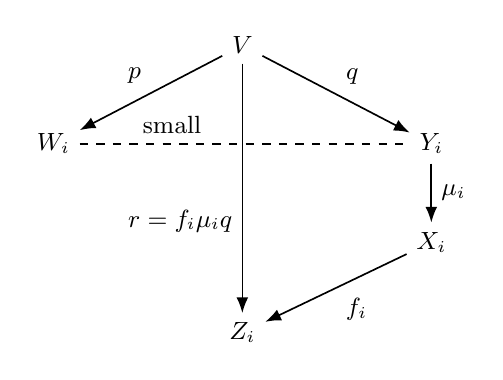
\begin{tikzpicture}[
   >=Latex,
   every node/.style={font=\small},
   map/.style={->,semithick}
 ]
  \node (V) at (0,2.5) {$V$};
  \node (Wi) at (-2.4,1.25) {$W_i$};
  \node (Yi) at (2.4,1.25) {$Y_i$};
  \node (Xi) at (2.4,0) {$X_i$};
  \node (Zi) at (0,-1.15) {$Z_i$};
  \draw[map] (V)--node[above left] {$p$}(Wi);
  \draw[map] (V)--node[above right] {$q$}(Yi);
  \draw[map] (Yi)--node[right] {$\mu_i$}(Xi);
  \draw[map] (Xi)--node[below right] {$f_i$}(Zi);
  \draw[map] (V)--node[left,pos=.63] {$r=f_i\mu_iq$}(Zi);
  \draw[dashed,semithick] (Wi)--node[above,pos=.28] {small}(Yi);
 \end{tikzpicture}
 \caption{The final comparison is made on $V$.
 The class $p^*P_{W_i}$ descends along $r$; no morphism from $W_i$
 to $X_i$ or to $Z_i$ is required.}
 \label{fig:perturbation-descent}
\end{figure}

The models $W_i$ and $Y_i$ are small modifications with the same
transformed boundary and b-data.  Their $Q_i$-classes are both nef.
Applying Lemma~\ref{lem:small-comparison} in both directions gives
\begin{equation}
 p^*Q_{i,W_i}=q^*Q_{i,Y_i}
            =s^*L_i(\lambda_i).
 \label{eq:equal-nef-pullbacks}
\end{equation}
Consequently this class has zero degree on every $r$-vertical curve.
For such a curve $C$, if $p(C)$ is a point then
$p^*P_{W_i}\cdot C=0$ immediately.  Otherwise the projection formula
and \eqref{eq:equal-nef-pullbacks} show that $p(C)$ is
$Q_{i,W_i}$-trivial.  Proposition~\ref{prop:trivial-perturbation}(4)
then gives $p^*P_{W_i}\cdot C=0$ as well.

The map $r$ is proper and birational.  Its target $Z_i$ is normal
compact Kähler with rational singularities by the ordinary-step
construction, and its source $V$ is smooth compact Kähler.
Its fibres are connected, and its general fibre is a point.
Thus all the hypotheses of Lemma~\ref{lem:pullback-image} apply to
$r$.  There is a class $\xi\in\BC(Z_i)$ with
\begin{equation}
 p^*P_{W_i}=r^*\xi.
 \label{eq:limiting-descent}
\end{equation}

We next form the ordinary canonical-and-boundary comparison.
Using compatible canonical data, the difference
\begin{equation}
 F=p^*(K_{W_i}+\Theta_{W_i})
          -s^*(K_{X_i}+\Delta_i)
 \label{eq:final-exceptional-divisor}
\end{equation}
is an actual real divisor on $V$, with the relative canonical terms
interpreted as in Section~\ref{sec:analytic}.
It is exceptional over $X_i$: on every prime that is not
$s$-exceptional the two boundary coefficients agree, since the
limiting boundary on $Y_i$ pushes to $\Delta_i$ and $W_i$ is small
to $Y_i$.  This constructs the divisor before any appeal to its
cohomology class.

By \eqref{eq:limiting-descent},
\[
 [F]=p^*P_{W_i}-s^*D_i
     =s^*(f_i^*\xi-D_i).
\]
Hence $F$ is numerically trivial over $X_i$.
Lemma~\ref{lem:negativity}, applied to $F$ and to $-F$, gives $F=0$.
Pullback injectivity for $s$ now yields
\[
 D_i=f_i^*\xi\quad\text{in }\BC(X_i).
\]
Its intersection with the ray contracted by $f_i$ is therefore zero,
contradicting the strict $D_i$-negativity with which that ray was chosen.
The scaling program is finite.
\end{proof}

\section{The two endpoints}\label{sec:endpoints}

The scaling program is finite by Proposition~\ref{prop:scaling-finite}.
We now identify its endpoint from the pseudo-effectivity of the original
adjoint.  Only ordinary birational comparisons are needed for this last step.

\begin{lemma}\label{lem:pe-step}
Let $(T,B)\dashrightarrow(T',B')$ be an ordinary negative divisorial
contraction or flip between normal compact Kähler klt pairs, with rational
boundaries and rational line-bundle adjoints.  Then $K_T+B$ is pseudo-effective if
and only if $K_{T'}+B'$ is pseudo-effective.
\end{lemma}

\begin{proof}
Set $D=K_T+B$ and $D'=K_{T'}+B'$.  The ordinary comparison in
Proposition~\ref{prop:ordinary-step} and Lemma~\ref{lem:negativity} gives,
on a common smooth compact Kähler resolution $p:V\to T$, $q:V\to T'$,
\[
 p^*D=q^*D'+F,\qquad F\geq0,
\]
where $F$ is an actual divisor exceptional over $T'$.
If $D'$ is pseudo-effective, its pullback plus $[F]$ is pseudo-effective;
descent along $p$ shows that $D$ is pseudo-effective.
Conversely, if $D$ is pseudo-effective, exceptional descent along $q$
applied to $q^*D'+[F]$ proves that $D'$ is pseudo-effective.
Both uses of pullback and descent are justified by
Lemma~\ref{lem:positive-descent}.
\end{proof}

\begin{lemma}\label{lem:mori-not-pe}
Let $g:Y\to S$ be a projective surjective morphism of normal compact Kähler
varieties with $\dim S<\dim Y$.  If a rational line bundle $D$ satisfies
$-D$ $g$-ample, then $D$ is not pseudo-effective.
\end{lemma}

\begin{proof}
Suppose that $c_1(D)$ contains a closed positive current $T$ with local
plurisubharmonic potentials.  Choose a point $y$ where such a potential is
finite and which lies on a positive-dimensional component of a fibre of
$g$.  This is possible on the dense open locus of fibres of the expected
dimension: the pole set of a plurisubharmonic potential contains no open
subset.  That fibre component is projective, so hyperplane sections through
$y$ give an integral curve $C$ through $y$ contained in the fibre.
Let $\nu:C^\nu\to Y$ denote its normalization followed by inclusion.

Local potentials pull back under $\nu$ to subharmonic functions or to the
constant $-\infty$.  Finiteness at a preimage of $y$ excludes the latter
alternative on the connected curve.  Thus they define a positive current
$\nu^*T$ in the class $\nu^*c_1(D)$, and
\[
 D\cdot C=\int_{C^\nu}\nu^*T\geq0.
\]
This contradicts $D\cdot C<0$, which follows from relative ampleness.
The choice of $y$ is essential: no restriction of $T$ to a curve contained
in its pole set has been used.
\end{proof}

\begin{proof}[Proof of Theorem~\ref{thm:finite}]
Run the scaling construction on the given pair $(X,\Delta)$.
Proposition~\ref{prop:ordinary-step} supplies each ordinary negative step,
and Proposition~\ref{prop:scaling-finite} proves that the construction
stops after finitely many such steps.  Write its endpoint as $(Y,\Gamma)$.
All intermediate varieties are normal compact Kähler fourfolds, all
boundaries are the rational transforms of $\Delta$, and all pairs remain
ordinary klt and globally Weil-divisor $\Q$-factorial with the stipulated
canonical datum.  The optional strong global property is preserved by the
same Proposition.  The auxiliary extractions used to prove finiteness do
not change this program, which starts on $X$ itself.

The stopping rule gives either a nef adjoint $K_Y+\Gamma$ or a Mori
contraction $g:Y\to S$.  In the latter case
Proposition~\ref{prop:ordinary-step} supplies a normal compact Kähler base,
a projective surjective morphism with connected fibres, $\dim S<4$,
relative numerical rank $\rho(Y/S)=1$, and relative ampleness of
$-(K_Y+\Gamma)$.  These are precisely the required Mori fibre space
conditions, with relative rank computed from global Cartier classes.
The same Proposition gives relative Bott--Chern dimension one for every
negative contraction, including $g$.

By Lemma~\ref{lem:pe-step}, the adjoint at every stage has the same
pseudo-effectivity status as $K_X+\Delta$.  If the latter is
pseudo-effective, Lemma~\ref{lem:mori-not-pe} excludes the Mori alternative,
so the endpoint is nef.  If it is not pseudo-effective, the endpoint
cannot be nef, since nef classes are pseudo-effective by
Lemma~\ref{lem:positive-descent}; hence the endpoint has the asserted Mori
fibre structure.

For completeness, the nef endpoint has the discrepancy properties of a
log minimal model.  No step extracts a divisor.  On a common resolution of
the finite sequence, with maps $p:V\to X$ and $q:V\to Y$, the ordinary
effective comparison divisors add to
\[
 p^*(K_X+\Delta)=q^*(K_Y+\Gamma)+F,
 \qquad F\geq0,
\]
with $F$ exceptional over $Y$.  Consequently, for every prime divisor $E$
over these models,
\[
 a(E,Y,\Gamma)\geq a(E,X,\Delta).
\]
If a prime divisor on $X$ is contracted, its discrepancy increases strictly
at the divisorial step that contracts its transform and never decreases
thereafter.  Thus the displayed inequality is strict for every such
prime.  Here $a$ denotes the log discrepancy, as throughout the paper.

If the initial adjoint is nef, the construction takes no steps; conversely,
a zero-step nef outcome requires the initial adjoint to be nef.  In the
non-pseudo-effective case a zero-step program is also allowed when the
first selected contraction already gives a Mori fibre structure on $X$.
This completes both endpoint assertions.
\end{proof}

\appendix
\section{Why analytic local factoriality is different}
\label{sec:local-convention}

Global Weil-divisor $\Q$-factoriality does not require every analytic local
ring to be $\Q$-factorial.  The distinction already occurs for projective
threefolds with one ordinary double point; see
\cite[Definition~5.1, Remark~(b)]{Reid}.  The following product example
explains why the stronger local requirement cannot be inserted into
Theorem~\ref{thm:finite}.

\begin{proposition}\label{prop:local-convention}
There is a smooth projective fourfold $X$ with pseudo-effective, non-nef
canonical divisor for which no ordinary $K_X$-negative program can reach a
nef model while keeping every model analytically locally
$\Q$-factorial.  Its unique possible first negative birational contraction
is divisorial.  Its target is nevertheless globally factorial and admits
a nef canonical divisor.
\end{proposition}

\begin{proof}
\emph{Construction.}
Let $b:B\to\Pbb^4$ be the blowup of a point, let
$H=b^*\cO_{\Pbb^4}(1)$, and let $F$ be the exceptional divisor.
The graph of projection from that point embeds $B$ in
$\Pbb^4\times\Pbb^3$, and the restriction of $\cO(1,1)$ is $2H-F$.
Thus $2H-F$ is very ample.  Since $H$ is globally generated,
\[
 6H-2F=2(2H-F)+2H
\]
is very ample as well.  Take a general smooth member
$U\in|6H-2F|$.
Its image $U_0\subset\Pbb^4$ is smooth away from the blown-up point.
The quadratic jets of the defining sextics at that point are arbitrary,
so a general member has a nondegenerate quadratic initial term.
The holomorphic Morse lemma identifies its unique singularity with
\[
 xy-zw=0.
\]
The restriction $\pi:U\to U_0$ resolves this node, with exceptional
quadric
\[
 E=F|_U\simeq\Pbb^1\times\Pbb^1,
 \qquad \cO_U(E)|_E=\cO_E(-1,-1).
\]
Adjunction gives
\begin{equation}\label{eq:local-example-canonical}
 K_U=H|_U+E,
\end{equation}
since $K_B=-5H+3F$.

Integral weak Lefschetz for the smooth ample threefold $U\subset B$
\cite[Section~7, Corollary~7.3]{MilnorMorse1963} gives
\[
 H^1(U,\Z)=0,
 \qquad H^2(U,\Z)=\Z[H|_U]\oplus\Z[E].
\]
This is the blowup calculation underlying the classical example in
\cite[Definition~5.1, Remark~(b)]{Reid}.
Let $C$ be a smooth elliptic curve and set $X=U\times C$.
Its canonical divisor is the pullback of \eqref{eq:local-example-canonical},
so is effective.  If $\ell$ is either ruling in $E\times\{c\}$, then
$K_X\cdot\ell=-1$; in particular $K_X$ is not nef.

\emph{All negative contractions have the same target.}
Put $D=E\times C$ and let $h=\{e\}\times C$ be a horizontal curve.
A curve not contained in $D$ has nonnegative degree against both the
effective divisor $D$ and the nef hyperplane pullback.  Thus every
$K_X$-negative curve lies in $D$.
The two rulings of $E$ have the same class in $H_2(U,\R)$: both have degrees
$0,-1$ against the displayed basis of $H^2(U,\R)$.
Künneth and $H^1(U,\R)=0$ now show that every integral curve
$\gamma\subset D$ has class
\begin{equation}\label{eq:local-example-curve}
 [\gamma]=a[\ell]+b[h],\qquad a,b\geq0.
\end{equation}
Here $a$ is the sum of the projection degrees to the two factors of
$E=\Pbb^1\times\Pbb^1$, and $b$ is the projection degree to $C$.
Moreover $K_X\cdot\gamma=-a$, so negativity means $a>0$.

Let $f:X\to Z$ be any nontrivial projective birational contraction with
connected fibres, normal compact Kähler target, and $-K_X$ relatively
ample.  Choose a Kähler class $\omega_Z$ and set $\alpha=f^*\omega_Z$.
For a curve, vanishing of its degree against $\alpha$ is equivalent to
being contracted by $f$.
In particular $\alpha\cdot\ell\geq0$ and $\alpha\cdot h>0$: the
horizontal curve cannot be contracted because $K_X\cdot h=0$.
A contracted curve $\gamma$ has the form
\eqref{eq:local-example-curve} with $a>0$, and
\[
 0=\alpha\cdot\gamma
   =a(\alpha\cdot\ell)+b(\alpha\cdot h).
\]
It follows that $b=0$ and $\alpha\cdot\ell=0$.
Thus all rulings in every $E\times\{c\}$ are contracted, and $f$ is not
small.

Set $q=\pi\times\id_C:X\to U_0\times C$.
Its nontrivial fibres are the quadrics $E\times\{c\}$, which are connected
by their rulings, so $f$ is constant on every $q$-fibre.
Conversely, every curve in an $f$-fibre has the form
\eqref{eq:local-example-curve} with $b=0$, and is contracted by $q$.
A connected projective fibre is connected by chains of curves, so $q$ is
constant on every $f$-fibre.  The two targets are isomorphic: the reduced
image of $(q,f)$ in their product projects properly, bijectively and
bimeromorphically to each normal target, hence finitely and isomorphically.
Therefore $q$ is the only possible first negative birational contraction.
It is divisorial, and its relative numerical rank is one because both
quadric rulings have the same nonzero numerical class.

\emph{Failure of analytic local $\Q$-factoriality.}
Near the singular locus of $U_0\times C$, consider the prime analytic
divisor
\[
 P=\{x=z=0\}\times\text{(a disk)}
   \ \subset\ \{xy-zw=0\}\times\text{(a disk)}.
\]
On the blowup of the singular axis, its strict transform meets each
exceptional quadric in a ruling line.  If $nP$ were Cartier near an axis
point for some integer $n>0$, its pullback would have the form
$n\widetilde P+kE_{\mathrm{exc}}$.
The associated line bundle restricts trivially to the quadric over that
point, because it is pulled back from a line bundle at a point.
On the other hand its restriction is
\[
 \cO_{\Pbb^1\times\Pbb^1}(n-k,-k),
\]
up to interchanging the factors.  Triviality forces $k=0$ and $n=0$, a
contradiction.  The target is not analytically locally $\Q$-factorial.
Since $K_X$ is not nef and there is no small negative contraction,
there is no permissible first step under that local convention.

\emph{Compatibility with the global convention.}
The same example has a valid one-step global program.  Indeed,
$-E$ is $\pi$-ample, so $-K_X$ is $q$-ample, and adjunction on $U_0$ gives
\[
 \cO_{U_0\times C}(K_{U_0\times C})
 \simeq\operatorname{pr}_1^*\cO_{U_0}(1),
\]
which is nef.  On the blowup of the node the exceptional divisor has log
discrepancy two; its smooth product with $C$ is a log resolution with the
same log discrepancy.  Hence the target is terminal, in particular klt.

It remains to check that the local divisor $P$ is not a global
factoriality obstruction.  The displayed integral cohomology of $U$ and
Hodge decomposition give $H^1(U,\cO_U)=H^2(U,\cO_U)=0$ and
$\Pic(U)=\Z[H|_U]\oplus\Z[E]$.
The exponential sequence and Künneth therefore give
\[
 \Pic(X)=\Z[H]\oplus\Z[D]\oplus\operatorname{pr}_C^*\Pic(C).
\]
Strict transform and divisor pushforward identify
\[
 \Cl(U_0\times C)=\Pic(X)/\Z[D].
\]
Every surviving class descends to a Cartier class, either from the
hyperplane bundle on $U_0$ or from a line bundle on $C$.
Chow's theorem makes every global analytic Weil divisor on this projective
target algebraic, so every such divisor is Cartier
\cite[Section~4, no.~19, Proposition~13]{SerreGAGA1956}.
GAGA identifies its global coherent
rank-one reflexive sheaves with algebraic divisorial sheaves, which are
therefore invertible as well
\cite[Section~3, no.~12, Theorems~2--3]{SerreGAGA1956}. The plane $P$ is defined only on an analytic
neighbourhood; it need not extend to a divisor on the whole compact space.
\end{proof}

\enlargethispage{2\baselineskip}
\bibliographystyle{amsplain}
\begingroup
\renewcommand{\baselinestretch}{0.95}
\bibliography{references}
\endgroup
\end{document}
